\documentclass[xcolor=table]{beamer}
\usetheme{default}
\usecolortheme{wolverine}
\usepackage{subfigure}
\usepackage{graphicx}
\usepackage{tabularx}
\usepackage{booktabs}
\usepackage{ragged2e}
\usepackage{caption}
\usepackage{adjustbox}


\setbeamercolor{normal text}{fg=white}
\setbeamercolor{caption name}{fg=yellow}
\definecolor{mybg}{RGB}{2, 61, 150}
\setbeamercolor{background canvas}{bg=mybg}
\setbeamercolor{itemize item}{fg=yellow}
\setbeamercolor{itemize item}{fg=yellow}
\setbeamercolor{itemize subitem}{fg=yellow}
\setbeamercolor{itemize subsubitem}{fg=yellow}
\setbeamertemplate{caption}{\color{yellow}\insertcaption}

\usefonttheme{professionalfonts}
\setbeamerfont{frametitle}{size=\large}
\setbeamerfont{normal text}{size=\large}

\beamertemplatenavigationsymbolsempty

\title{D.S.P. based Field Oriented Control of Induction motor}
\author{Adhithya S 200901002\\Anabhayan S P 200901008}
\date{Under the guidance of Dr S Rama Reddy \\ Dean - Electrical sciences \vspace{0.3in}\\                  {\small\textit{Department of Electrical and Electronics Engineering\\Rajalakshmi Engineering college}}}

\usepackage{tikz}

\usetikzlibrary{shapes.geometric, arrows}

\setbeamercolor{itemize item}{fg=yellow}
 % Keep your preamble

\begin{document}

% Slide 1: Title Slide (keep as is)
\begin{frame}{}
	\maketitle
\end{frame}

\begin{frame}{Field Oriented Control}
	\begin{itemize}
		\item Add awesome images for indicating concept of FOC.
	\end{itemize}
\end{frame}


\begin{frame}
	\frametitle{Advantages of Vector Control in Induction Motors}
	\begin{itemize}
		\item \textbf{Dynamic Response:} Faster and more accurate response to changes.
		\item \textbf{Efficiency:} Reduced energy consumption and increased performance.
		\item \textbf{Speed Control:} Precise and accurate control of motor's speed.
		\item \textbf{Starting Torque:} High initial force for heavy-duty applications.
		\item \textbf{Regenerative Capability:} Energy recovery through regenerative braking.
	\end{itemize}
\end{frame}


% Slide 2: Block Diagram of FOC
\begin{frame}{Block Diagram of Field Oriented Control}
	\begin{figure}
		\centering

		\fbox{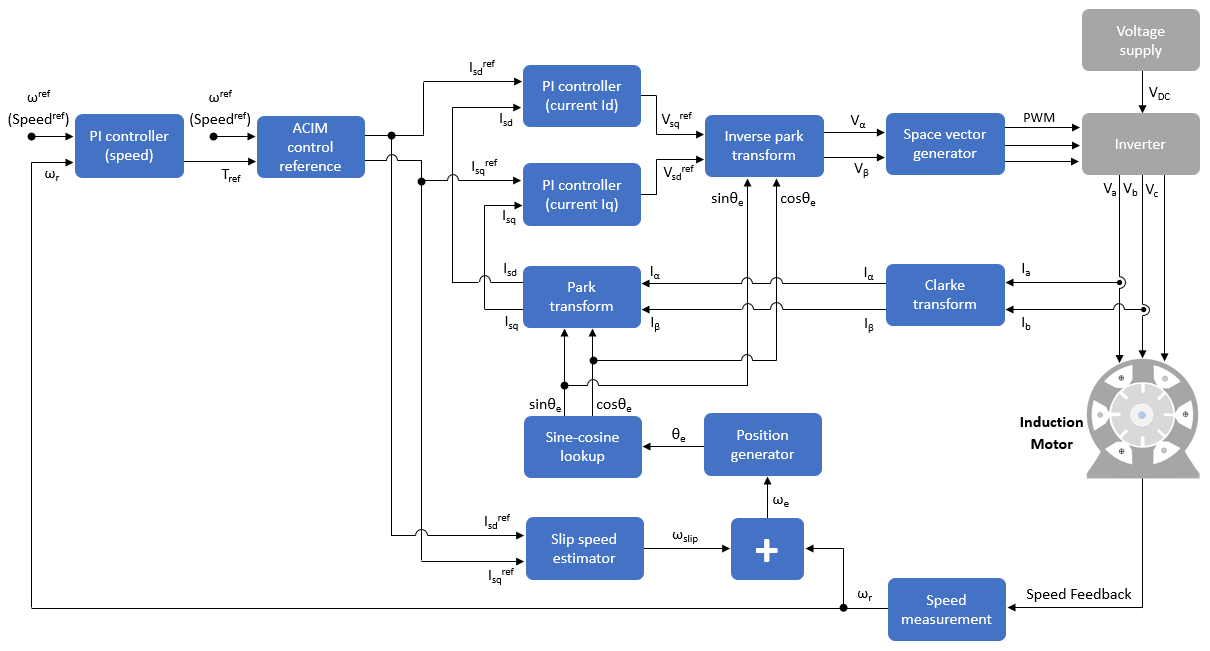
\includegraphics[width=4in]{sections/section2/images/blockDiagram.png}}
		\caption{Block Diagram of Field Oriented Control}
	\end{figure}
	\begin{itemize}
		\item Coordinate Transformations.
		\item PI Controllers.
		\item PWM Generation.
	\end{itemize}
\end{frame}

% Slide 3: Block Diagram of the System
\begin{frame}{Block Diagram of the System}
	\begin{figure}
		\centering

		\fbox{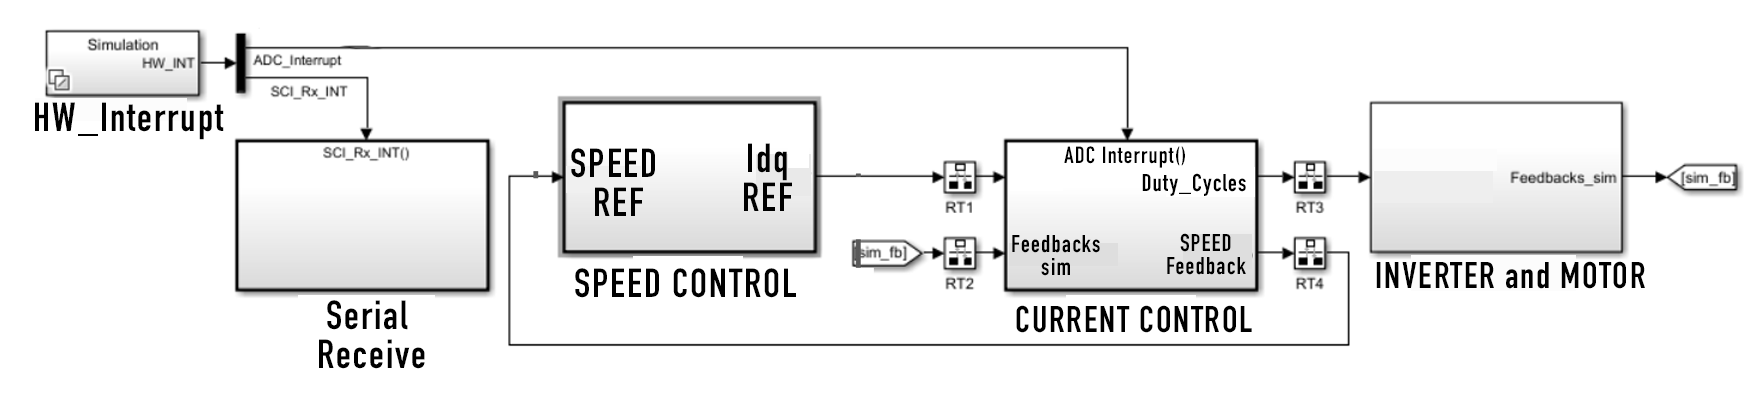
\includegraphics[width=4in]{sections/section3/images/simulation/blockDia.png}}
		\caption{Block Diagram of the System}
	\end{figure}
\end{frame}

% Slide 4: Speed Control Subsystem
\begin{frame}{Speed Control Subsystem}
	\begin{figure}
		\centering

		\fbox{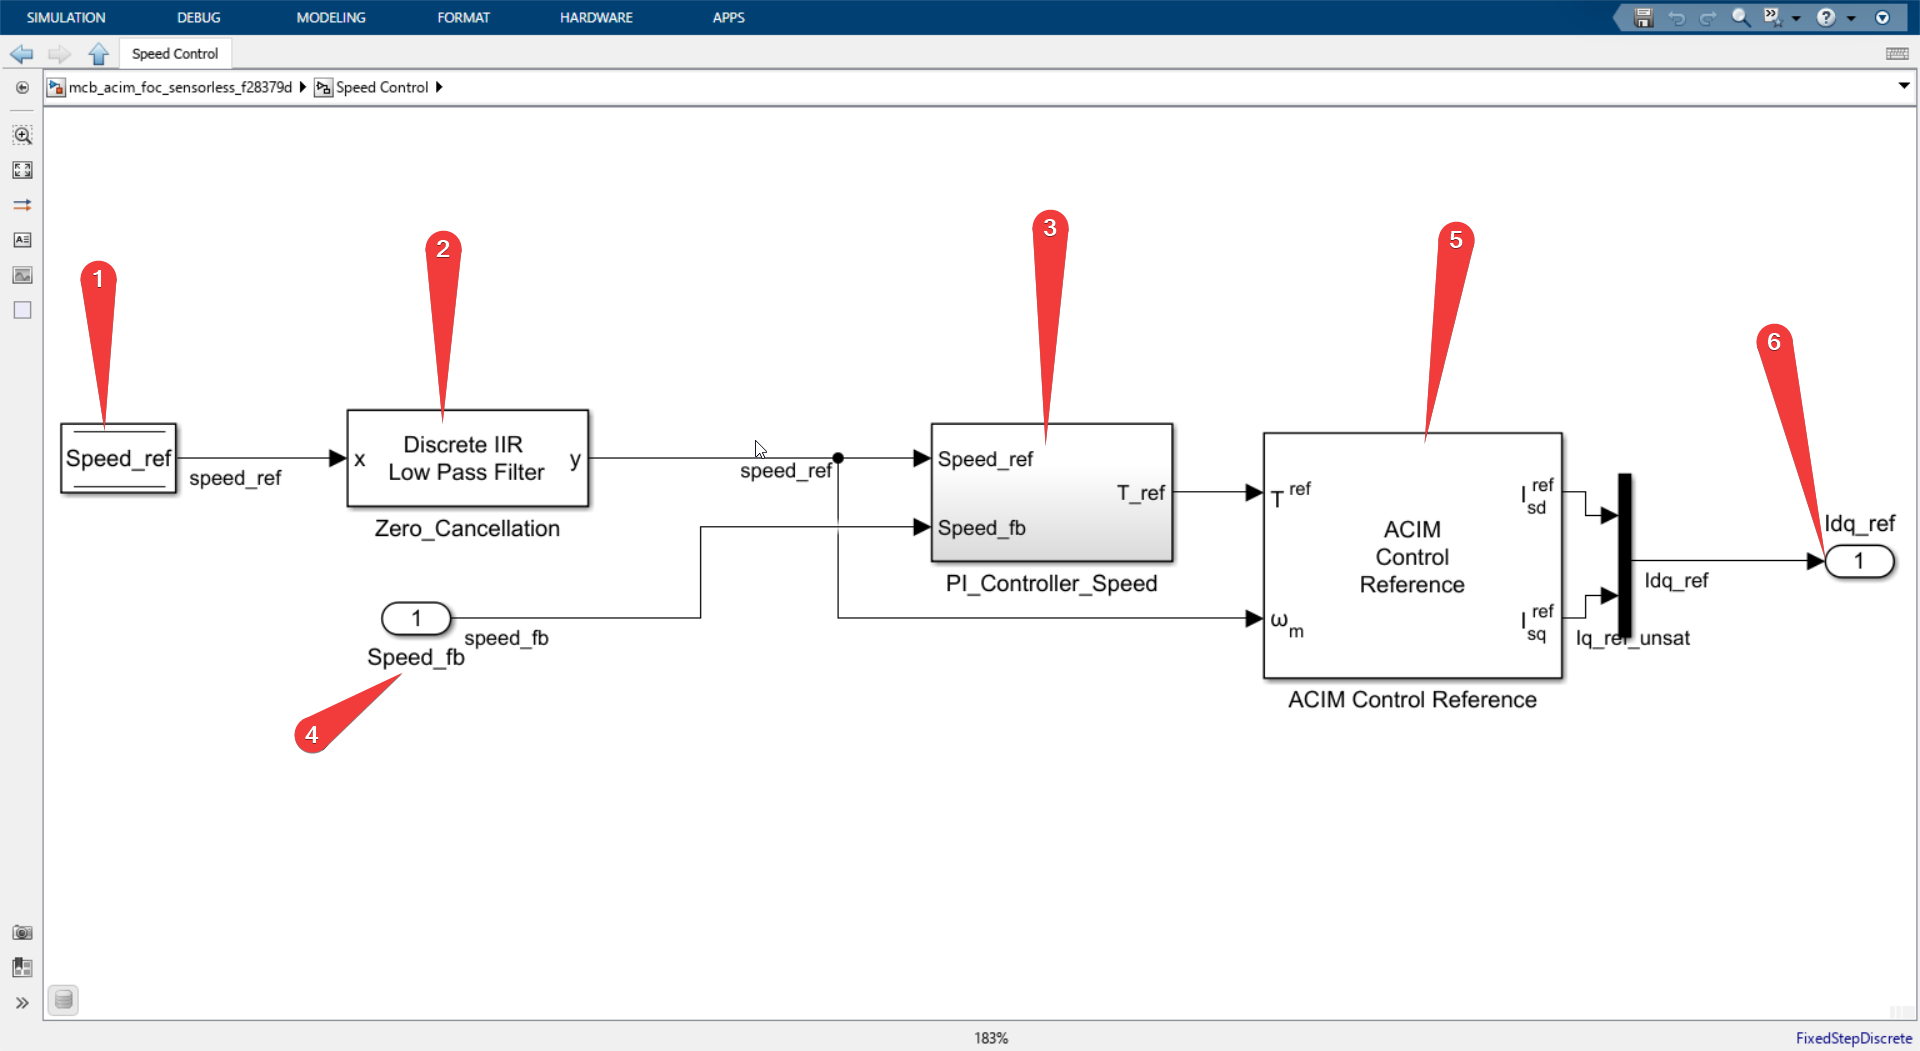
\includegraphics[width=4in]{sections/section3/images/simulation/speedControl/speedController.png}}
		\caption{Speed Control Subsystem}
	\end{figure}
\end{frame}

% Slide 5: Current Measurement
\begin{frame}{Current Measurement}
	\begin{figure}
		\centering

		\fbox{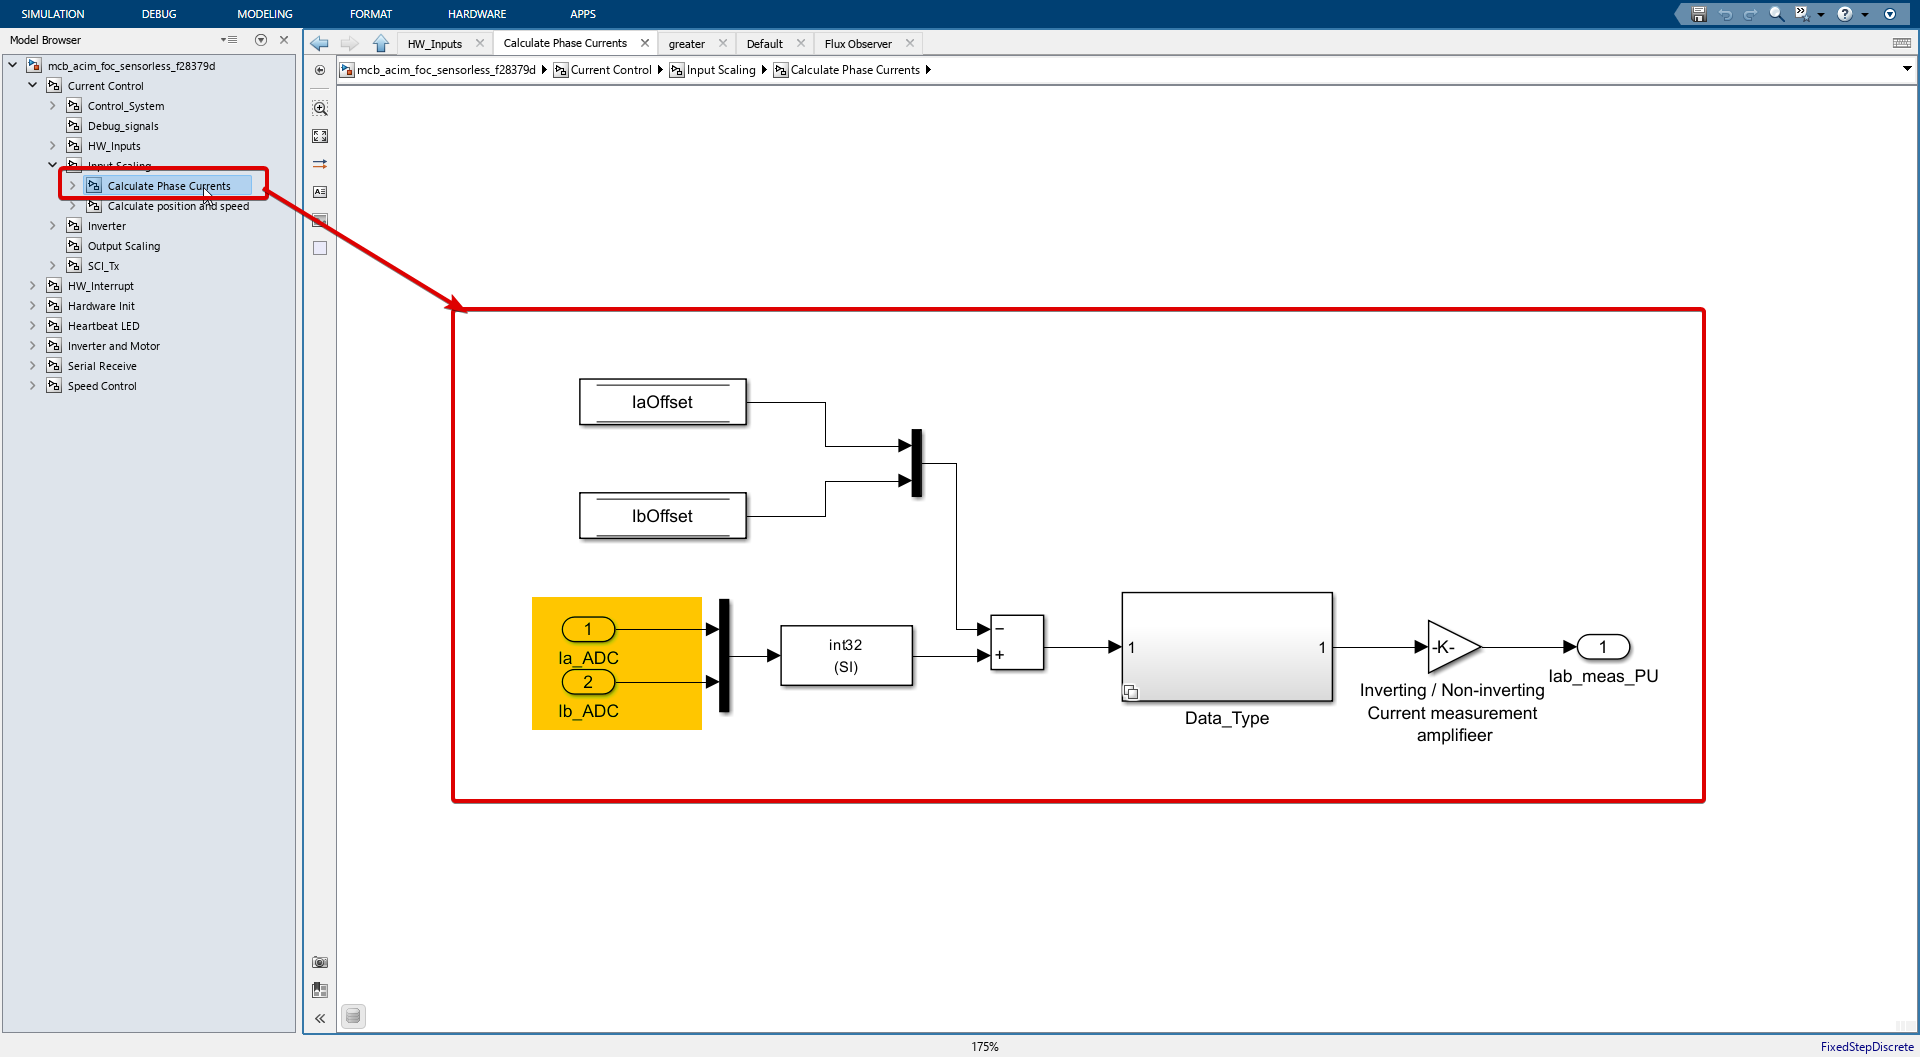
\includegraphics[width=4in]{sections/section3/images/simulation/inputScaling/currentMeasurement.png}}
		\caption{Current Measurement}
	\end{figure}
\end{frame}

% Slide 6: Position and Speed Estimation
\begin{frame}{Position and Speed Estimation}
	\begin{figure}
		\centering

		\fbox{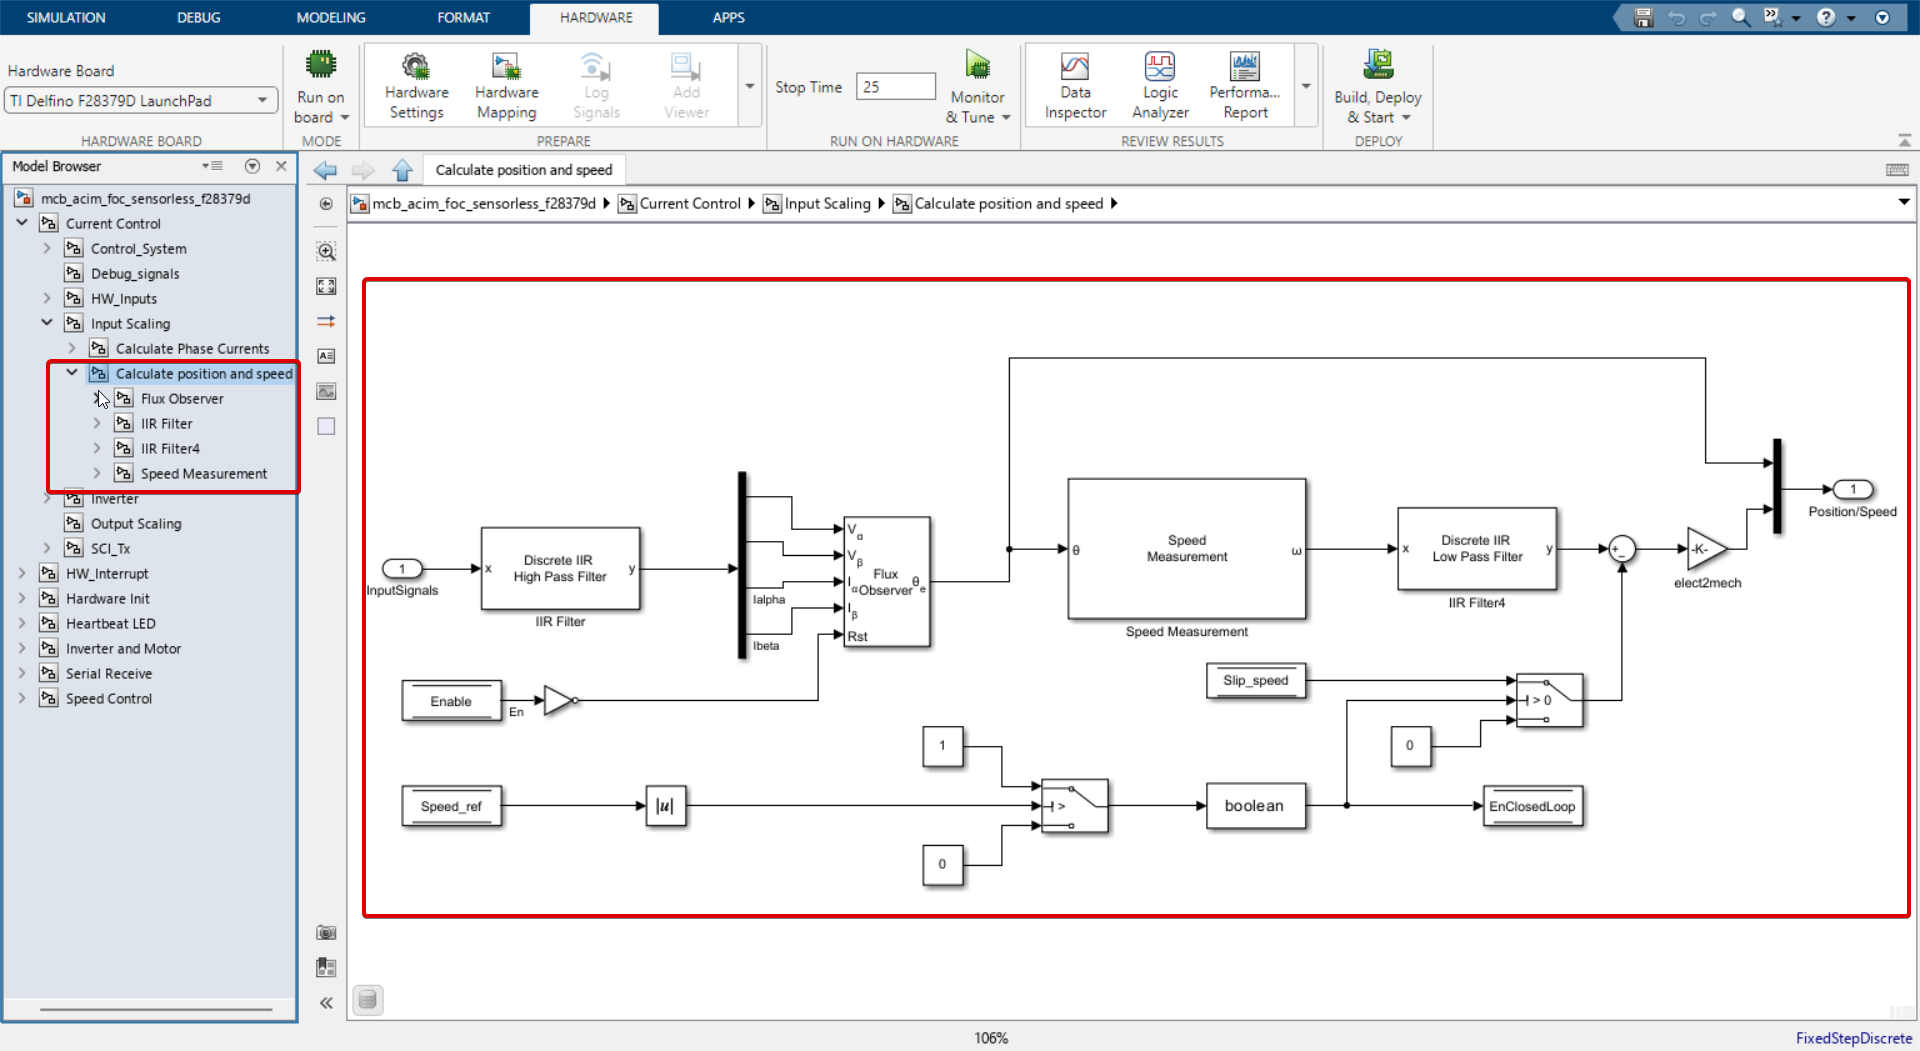
\includegraphics[width=4in]{sections/section3/images/simulation/inputScaling/fluxObserver.png}}
		\caption{Position and Speed Estimation}
	\end{figure}
\end{frame}

% Slide 7: Current Control System
\begin{frame}{Current Control System}
	\begin{figure}
		\centering

		\fbox{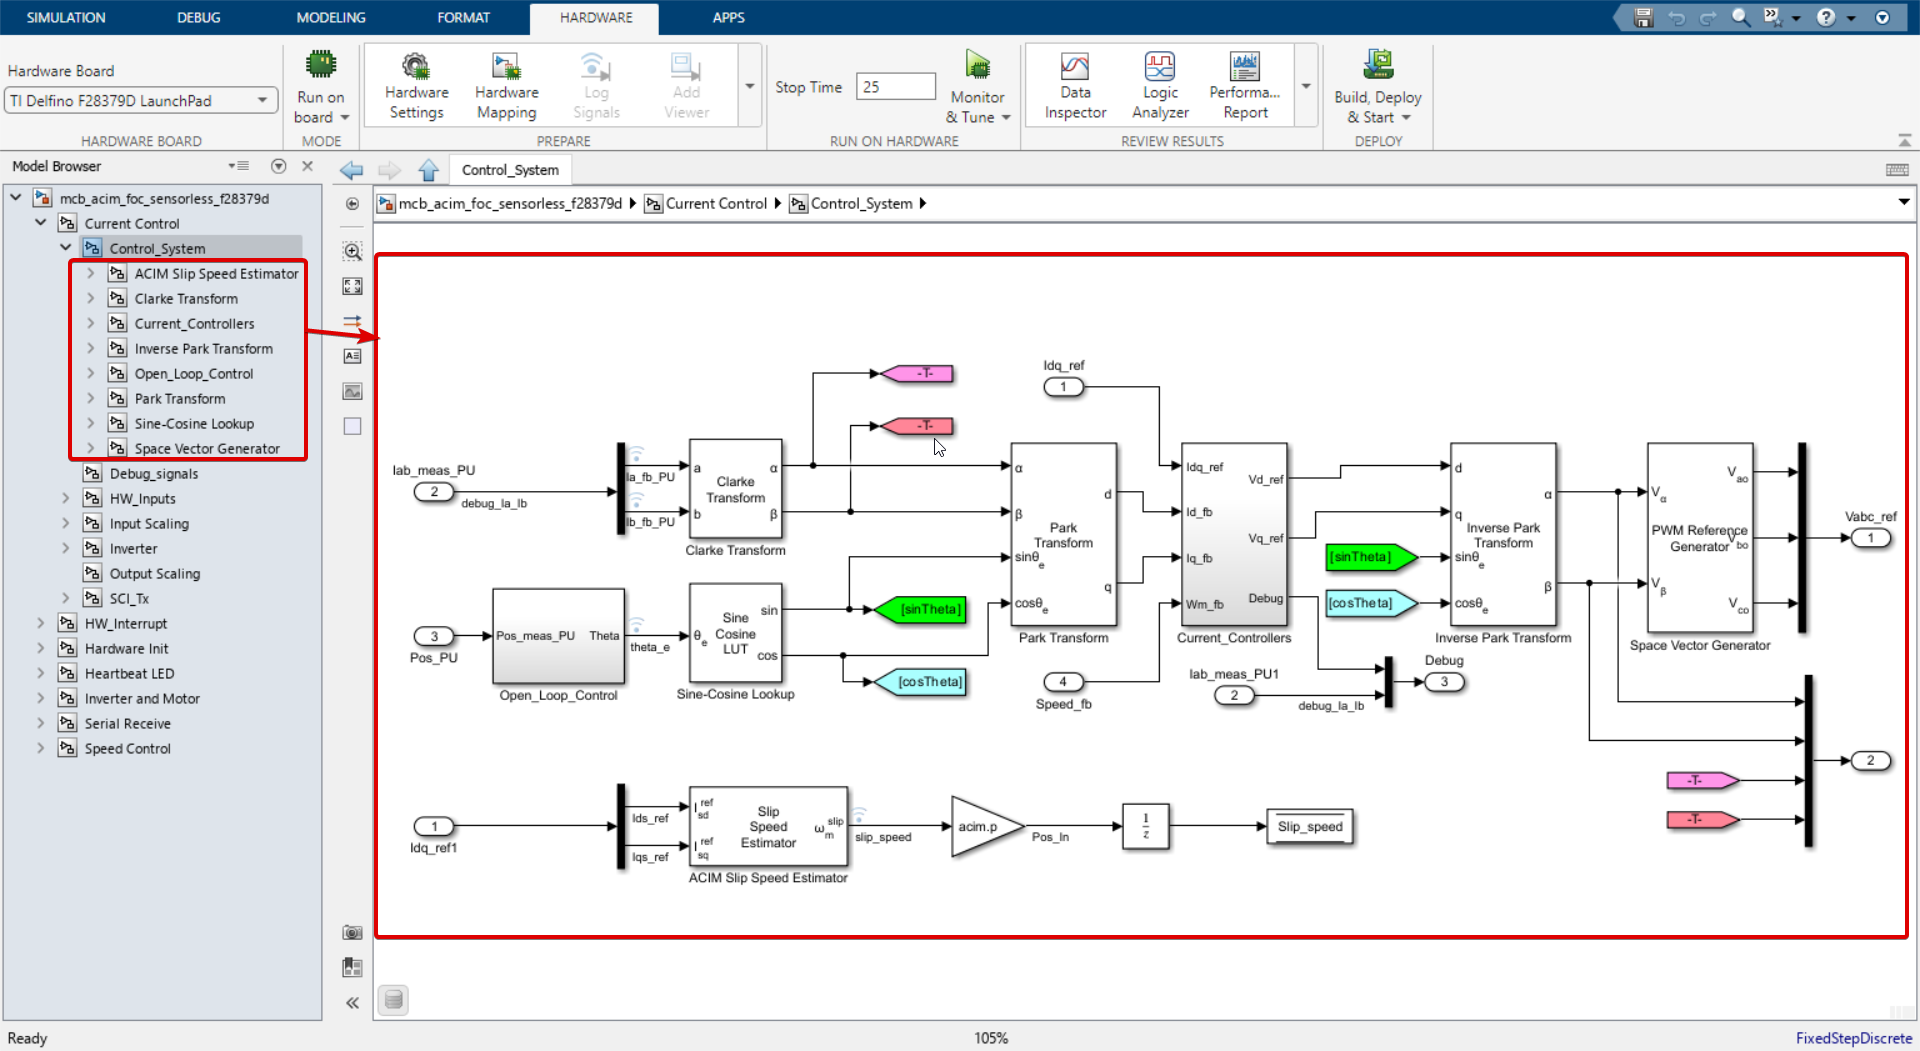
\includegraphics[width=4in]{sections/section3/images/simulation/currentControl/controlSystem.png}}
		\caption{Current Control System}
	\end{figure}
\end{frame}

% Slide 8: Speed Response
\begin{frame}{Speed Response}
	\begin{figure}
		\centering

		\fbox{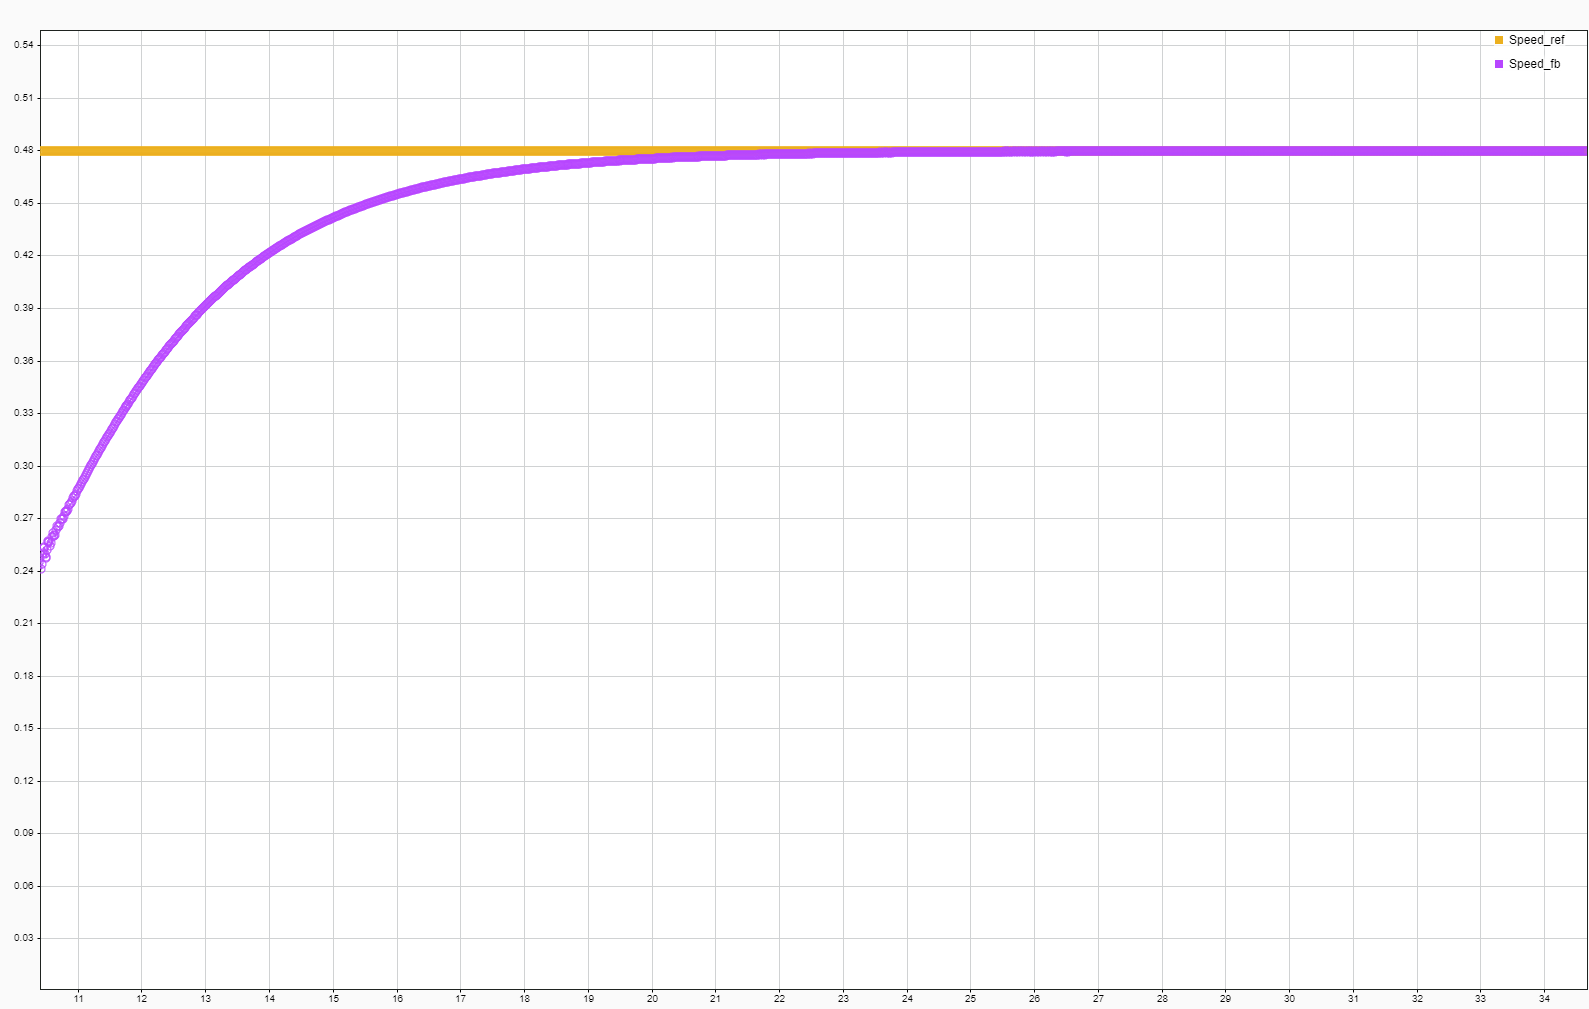
\includegraphics[width=4in]{sections/section3/images/simulationResutls/SpeedTrackingNoCursor.png}}
		\caption{Speed Response}
	\end{figure}
\end{frame}

% Slide 9: Slip Speed
\begin{frame}{Slip Speed}
	\begin{figure}
		\centering

		\fbox{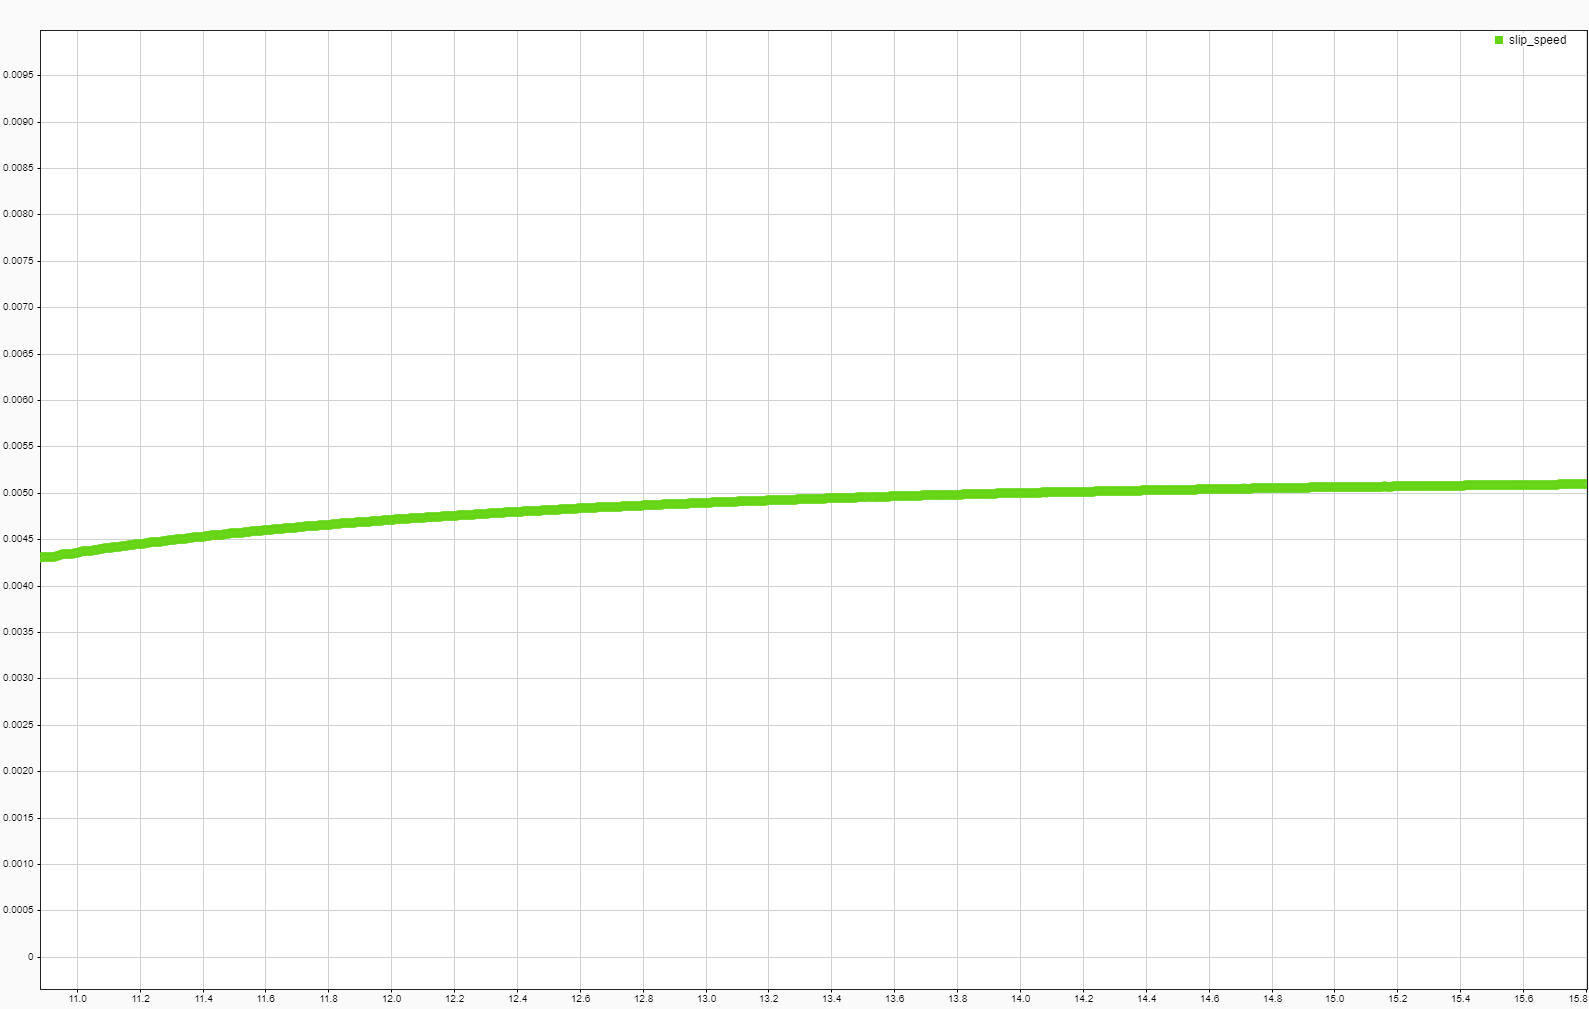
\includegraphics[width=4in]{sections/section3/images/simulationResutls/SlipSpeed.png}}
		\caption{Slip Speed}
	\end{figure}
\end{frame}

\begin{frame}{Ia and Ib Feedback/Measured Currents}
	\begin{figure}
		\centering

		\fbox{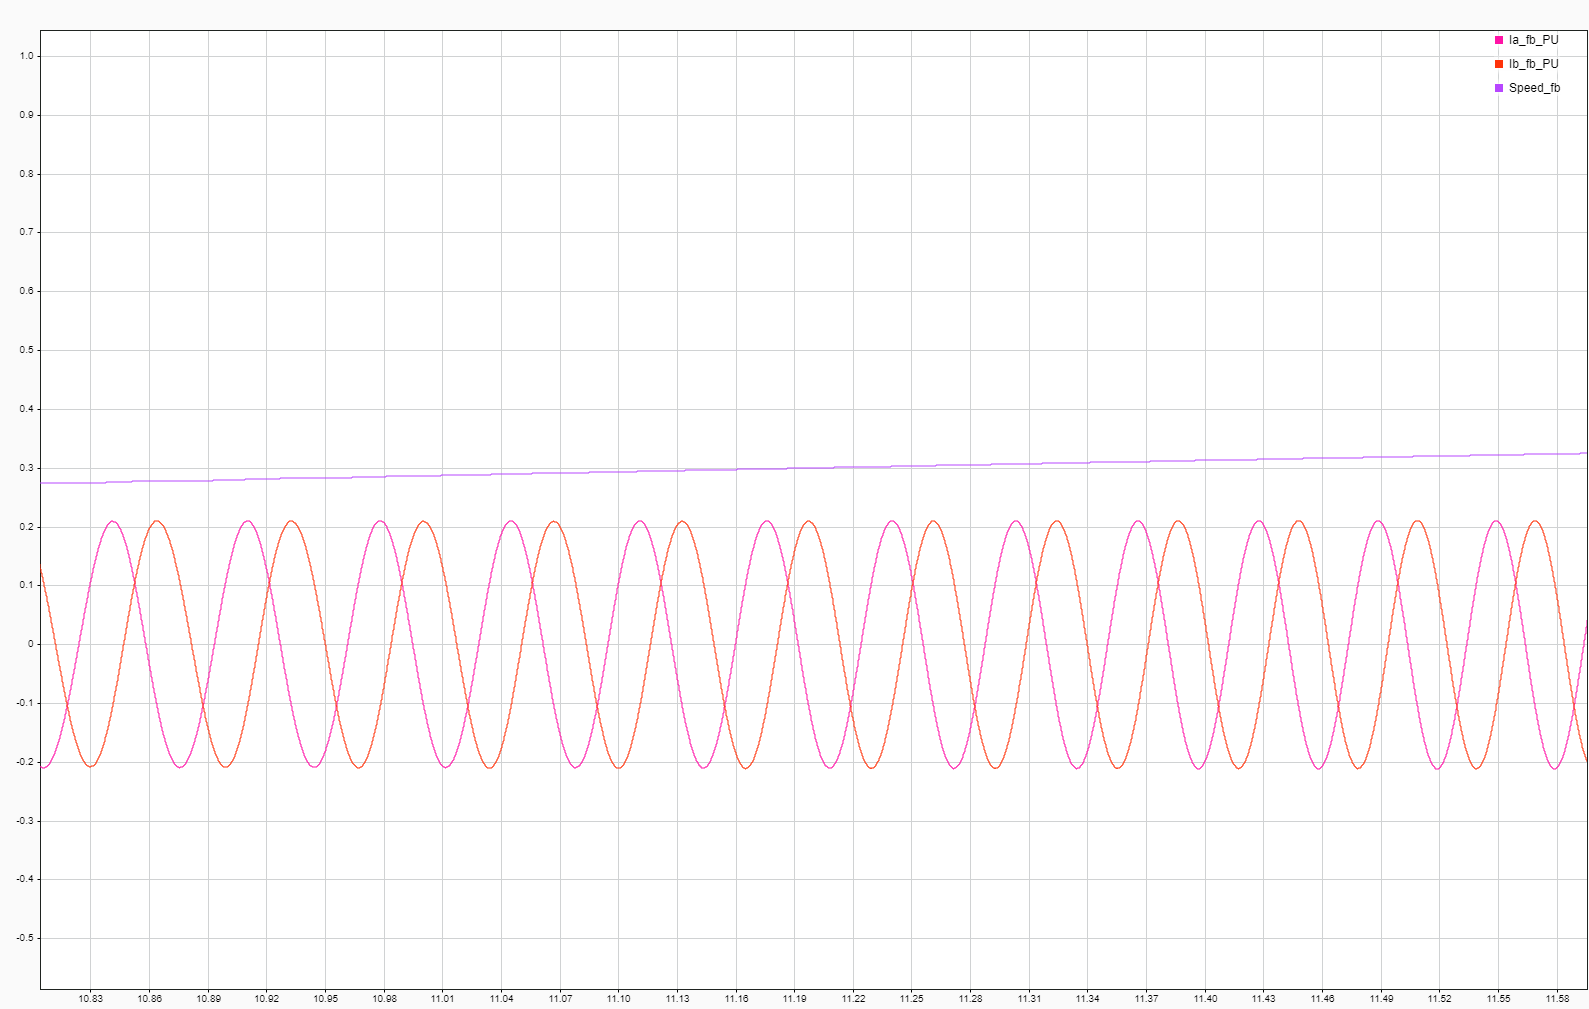
\includegraphics[width=4in]{sections/section3/images/simulationResutls/Ia_Ib_fb.png}}
		\caption{Ia and Ib Feedback/Measured Currents}
	\end{figure}
\end{frame}

% Slide 11: Id and Iq Reference Currents
\begin{frame}{Id and Iq Reference Currents}
	\begin{figure}
		\centering

		\fbox{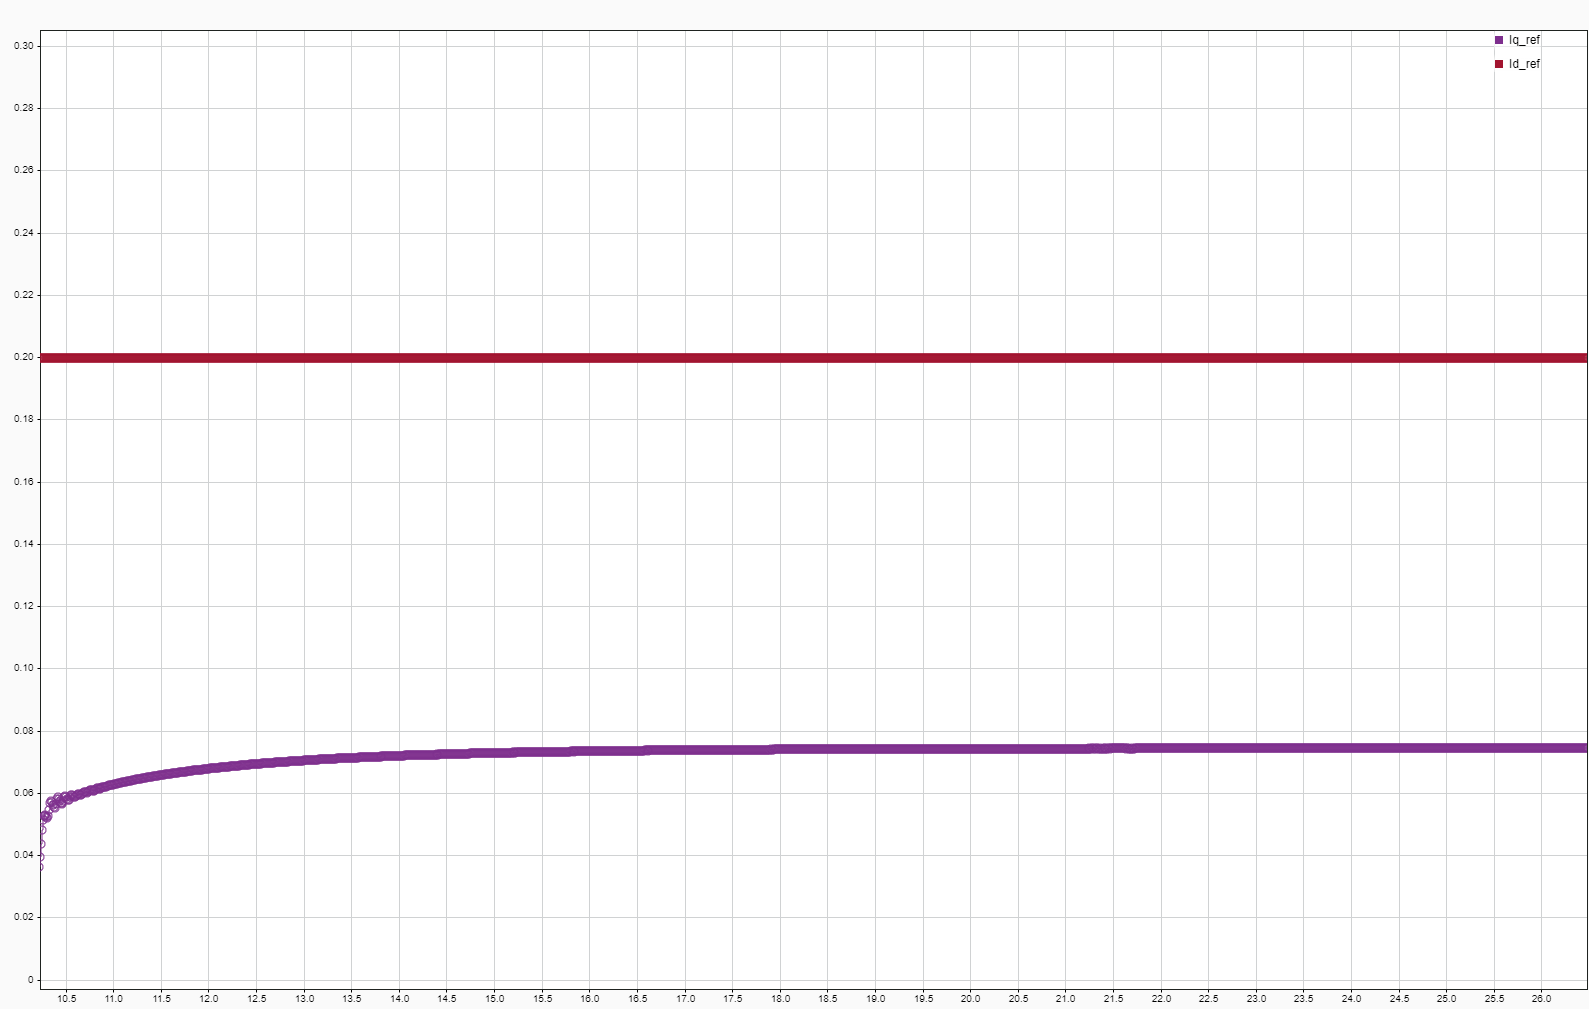
\includegraphics[width=4in]{sections/section3/images/simulationResutls/Id_ref_Iq_ref.png}}

		\caption{Id and Iq Reference Currents}
	\end{figure}
\end{frame}

% Slide 12: Id and Iq Feedback Currents
\begin{frame}{Id and Iq Feedback Currents}
	\begin{figure}
		\centering

		\fbox{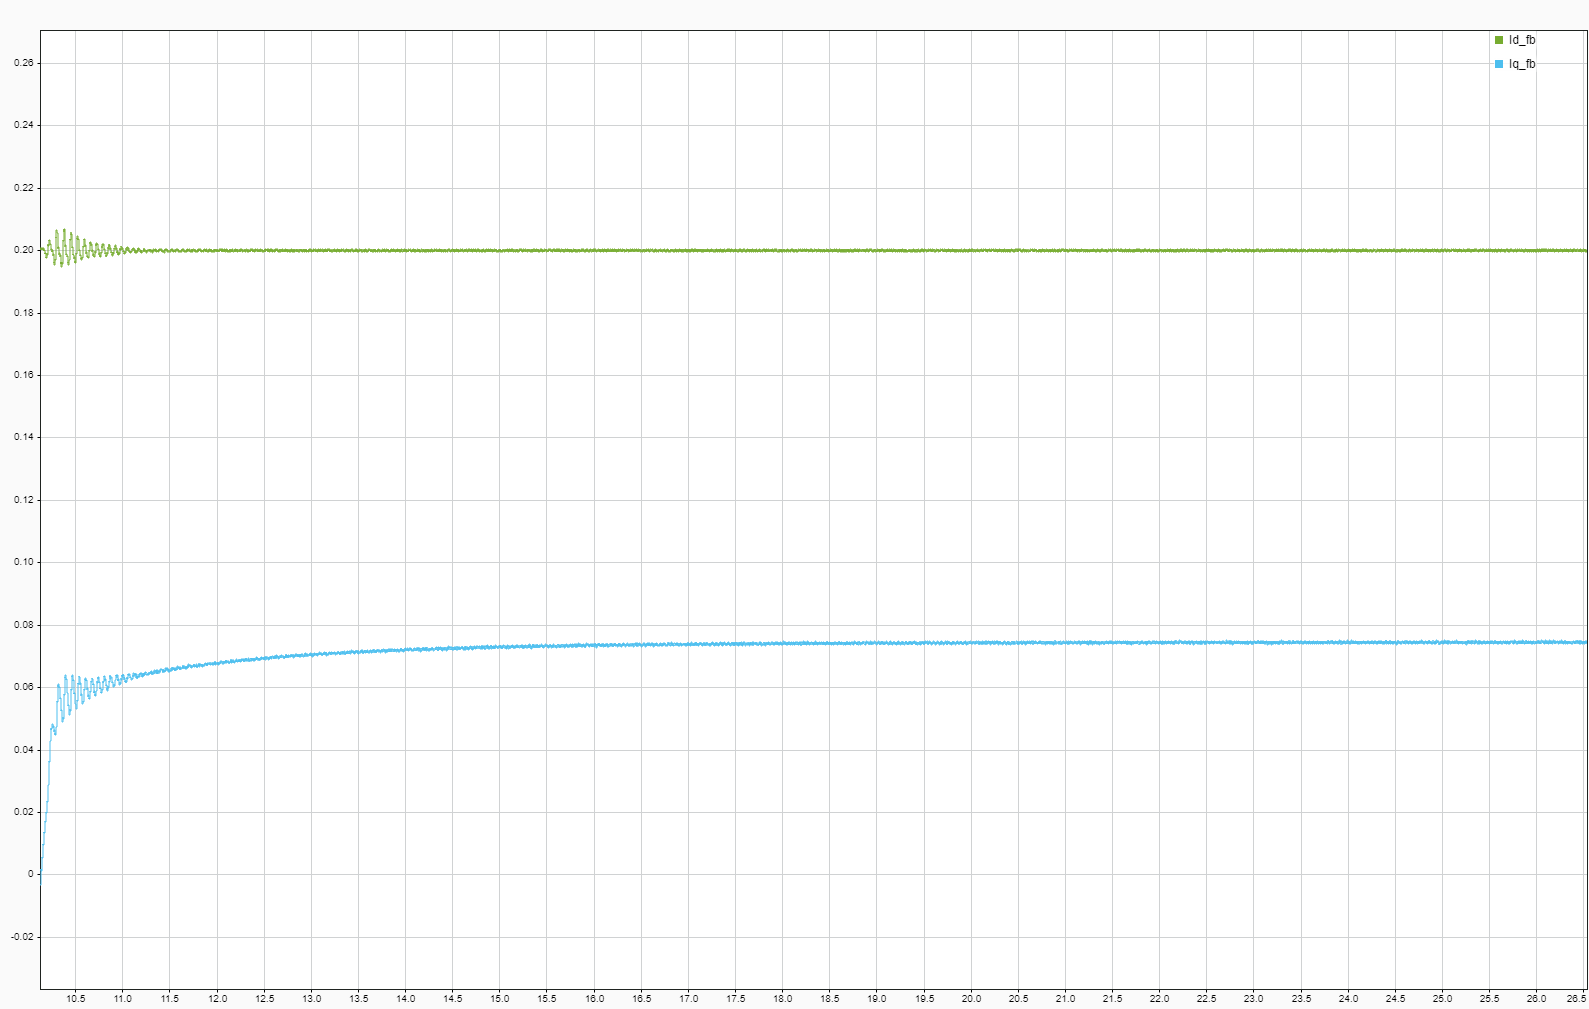
\includegraphics[width=4in]{sections/section3/images/simulationResutls/Id_fb_Iq_fb.png}}

	\end{figure}
\end{frame}

% Slide 13: Iq Reference and Feedback Currents (Torque producing current)
\begin{frame}{Iq Reference and Feedback Currents (Torque producing current)}
	\begin{figure}
		\centering

		\fbox{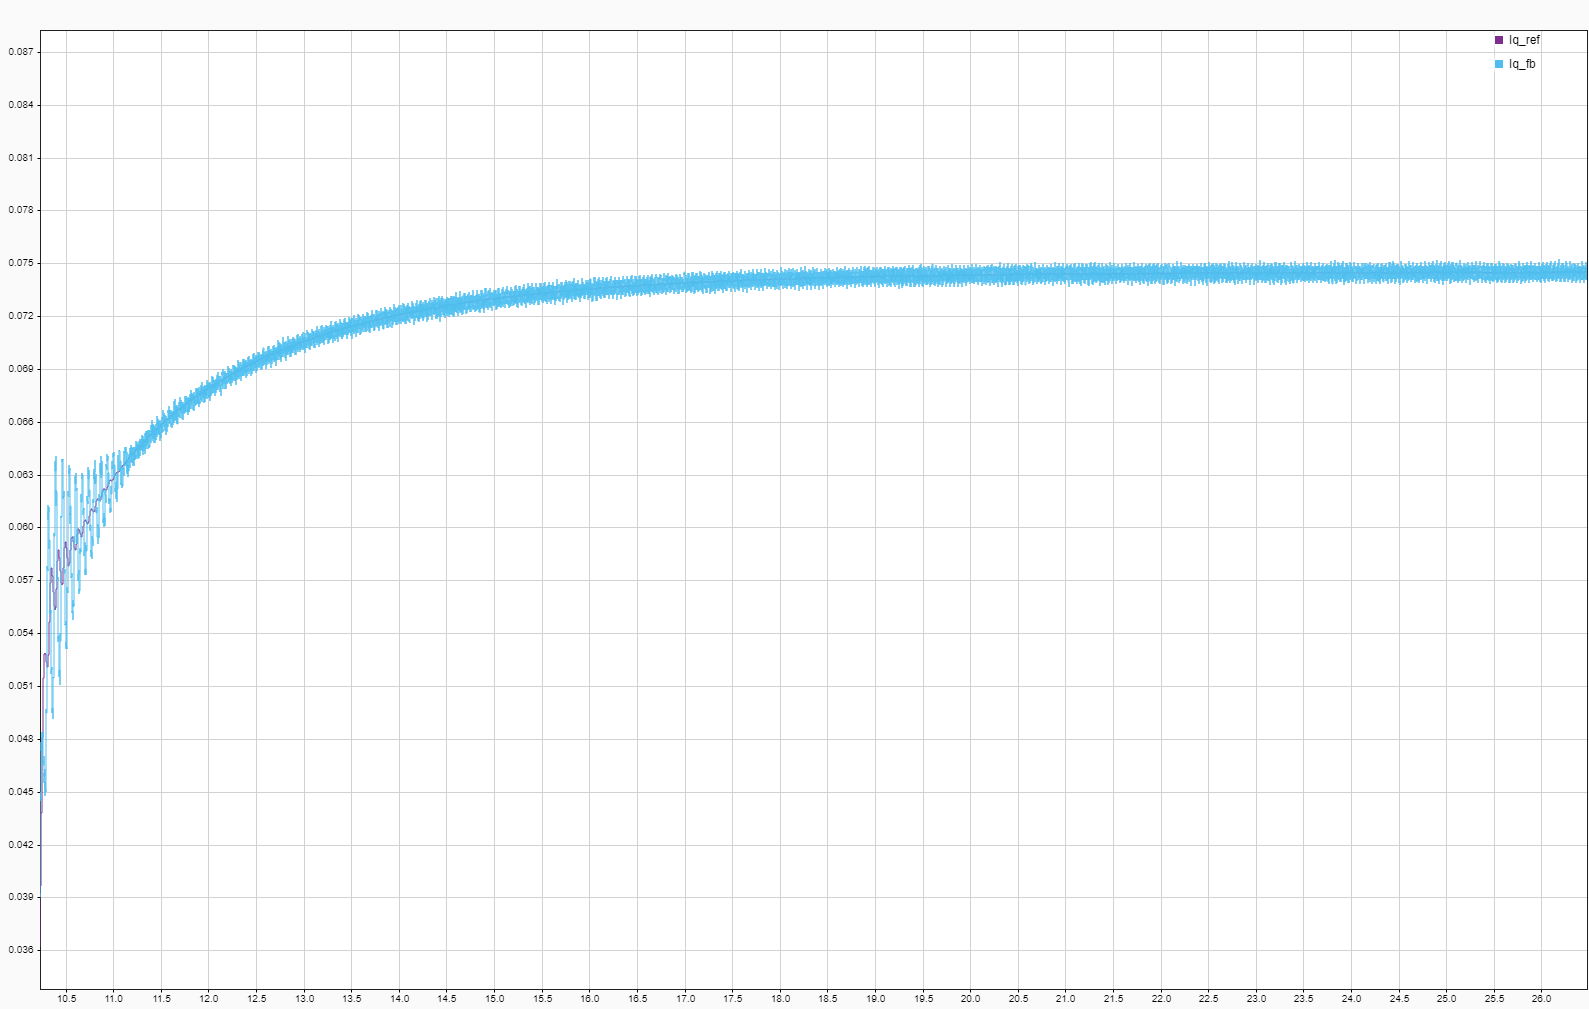
\includegraphics[width=4in]{sections/section3/images/simulationResutls/Iq_ref_fb.png}}

	\end{figure}
\end{frame}

% Slide 14: Id Reference and Feedback Currents (Magnetizing current)
\begin{frame}{Id Reference and Feedback Currents (Magnetizing current)}
	\begin{figure}
		\centering

		\fbox{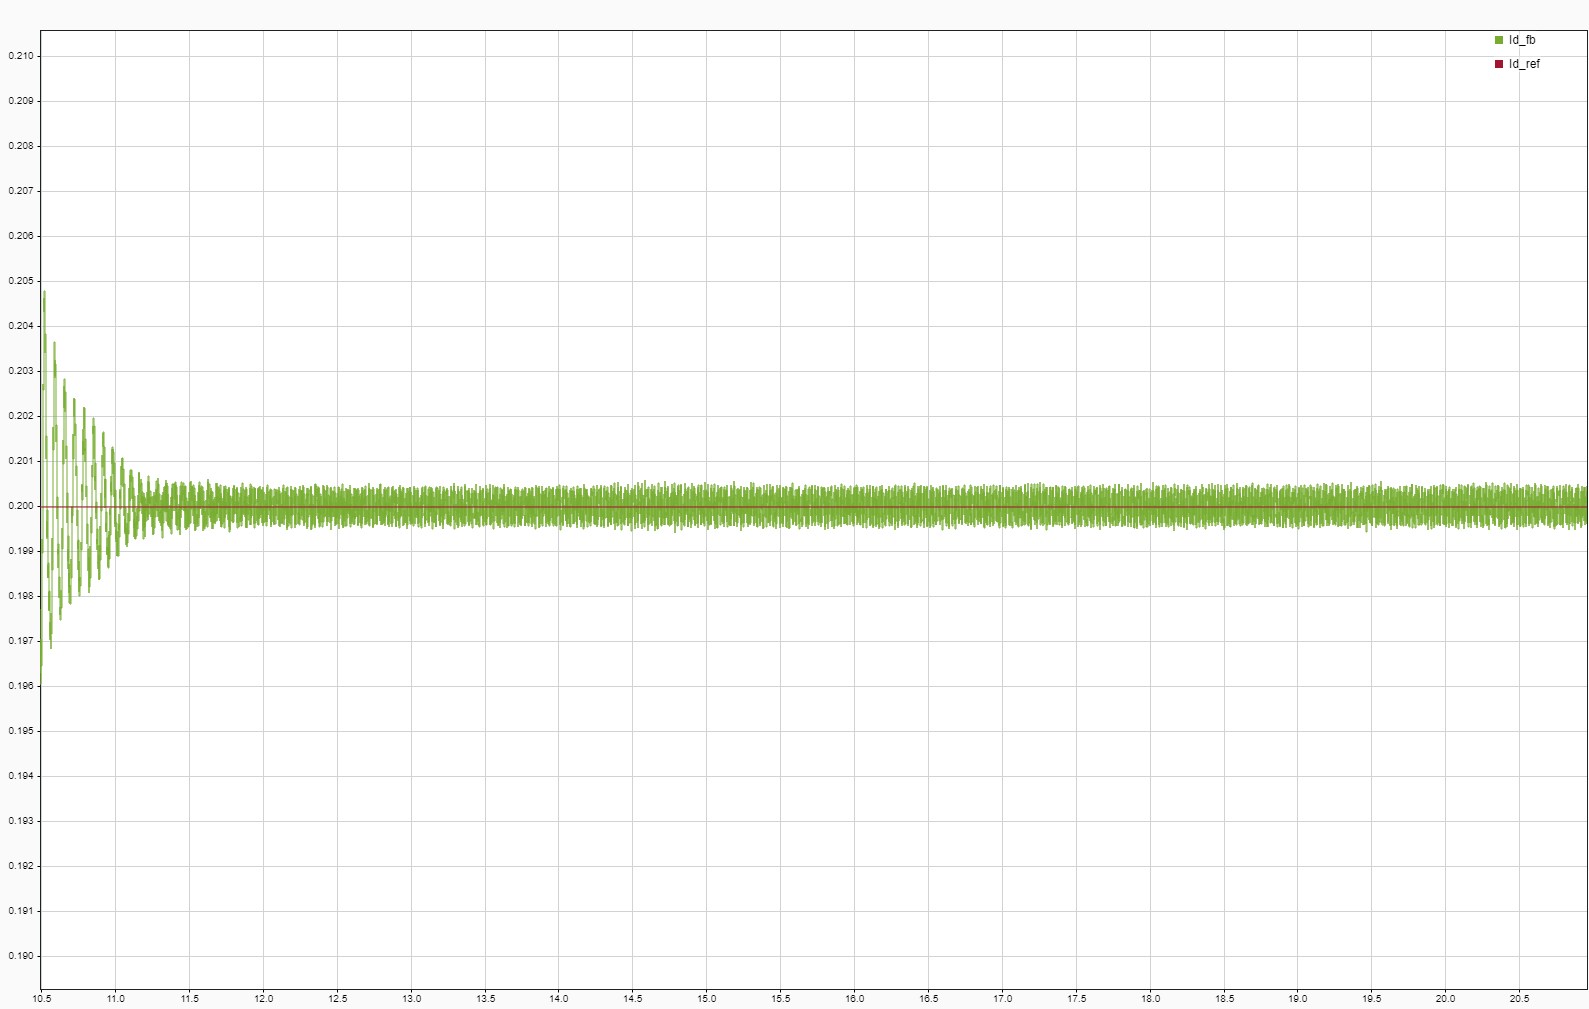
\includegraphics[width=4in]{sections/section3/images/simulationResutls/Id_ref_fb.png}}

	\end{figure}
\end{frame}

\begin{frame}{C2000 Features for Implementing Vector Control Algorithm}
	\begin{columns}
		\column{0.5\textwidth}
		\begin{figure}
			\centering
			\fbox{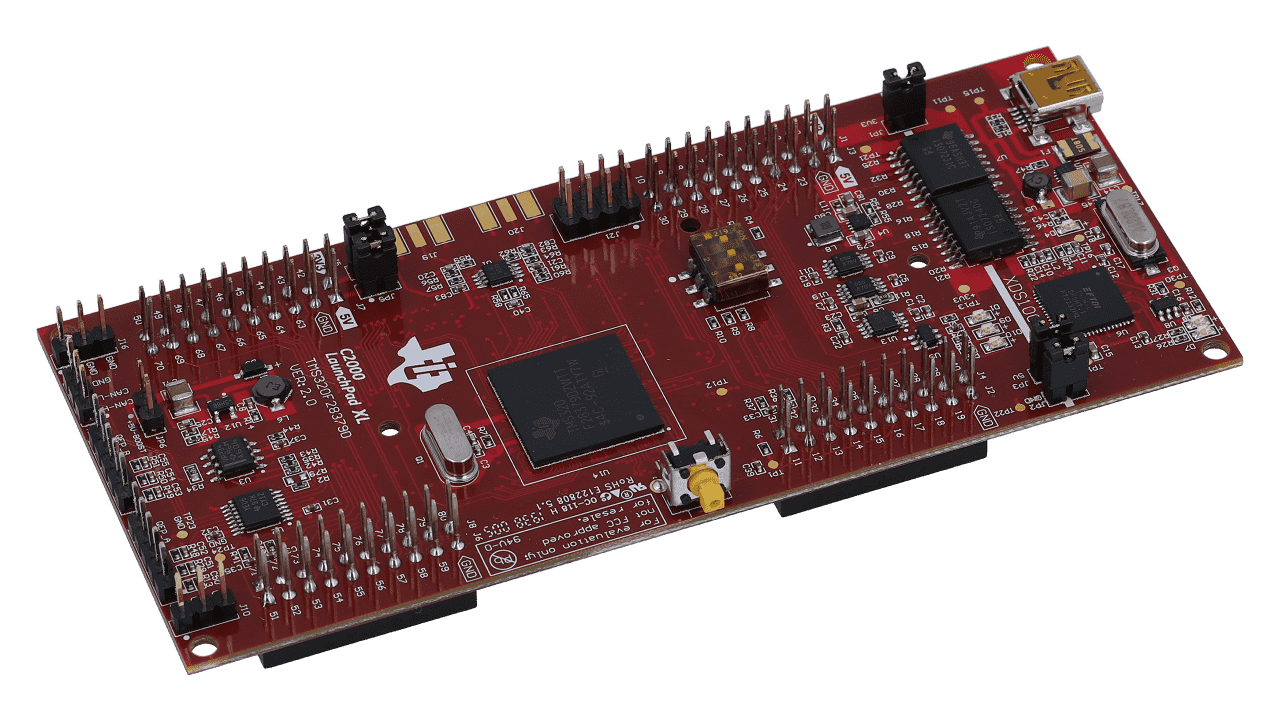
\includegraphics[width=2in]{sections/section4/images/f23879d/launchxl-f28379d-angled.png}}
			\caption{F28379D Launchpad}
		\end{figure}
		\column{0.5\textwidth}
		\begin{itemize}
			\item \textbf{Dual-Core C28x Architecture:} Enables simultaneous execution of control tasks and communication tasks, improving overall system performance.
			\item \textbf{Control Law Accelerator (CLA):} Offloads the CPU by executing time-critical control algorithms, freeing the CPU for other tasks.
			\item \textbf{High-Resolution PWM:} Offers precise control over motor's speed and torque, critical for effective Field Oriented Control (FOC).
			\item \textbf{Integrated ADCs:} Facilitates accurate and efficient sensing of motor currents and voltages, a key requirement in FOC.
			\item \textbf{Floating Point Unit:} Simplifies the implementation of complex mathematical algorithms used in FOC.
		\end{itemize}
	\end{columns}
\end{frame}


\begin{frame}{Advantages of Using Intelligent Power Module FSAM20SH60A}
	\begin{columns}
		\column{0.5\textwidth}
		\begin{figure}
			\centering
			\fbox{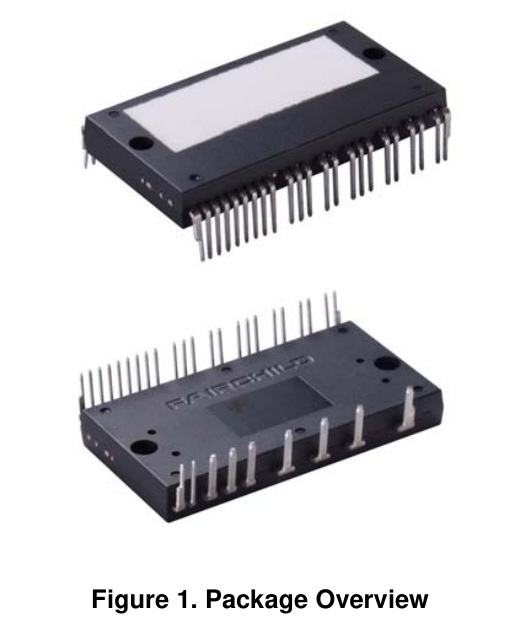
\includegraphics[width=0.9in]{sections/section4/images/IPM/ipm.png}}
			\caption{Intelligent Power Module FSAM20SH60A}
		\end{figure}
		\column{0.5\textwidth}
		\begin{itemize}
			\item \textbf{Compact Design:} Integrates power devices, drivers, and protection circuitry in a single package, saving space and simplifying system design.
			\item \textbf{Enhanced Performance:} Optimized for high-speed switching, reducing switching losses and improving overall efficiency.
			\item \textbf{Protection Features:} Includes built-in under-voltage lockout, over-temperature protection, and fault reporting, enhancing system reliability.
			\item \textbf{Ease of Use:} Simplifies system design and reduces time-to-market compared to designing with discrete components.
			\item \textbf{Cost-Effective:} Reduces the number of required components, lowering overall system cost.
		\end{itemize}
	\end{columns}
\end{frame}

\begin{frame}{Induction Motor}
	\begin{figure}
		\centering

		\fbox{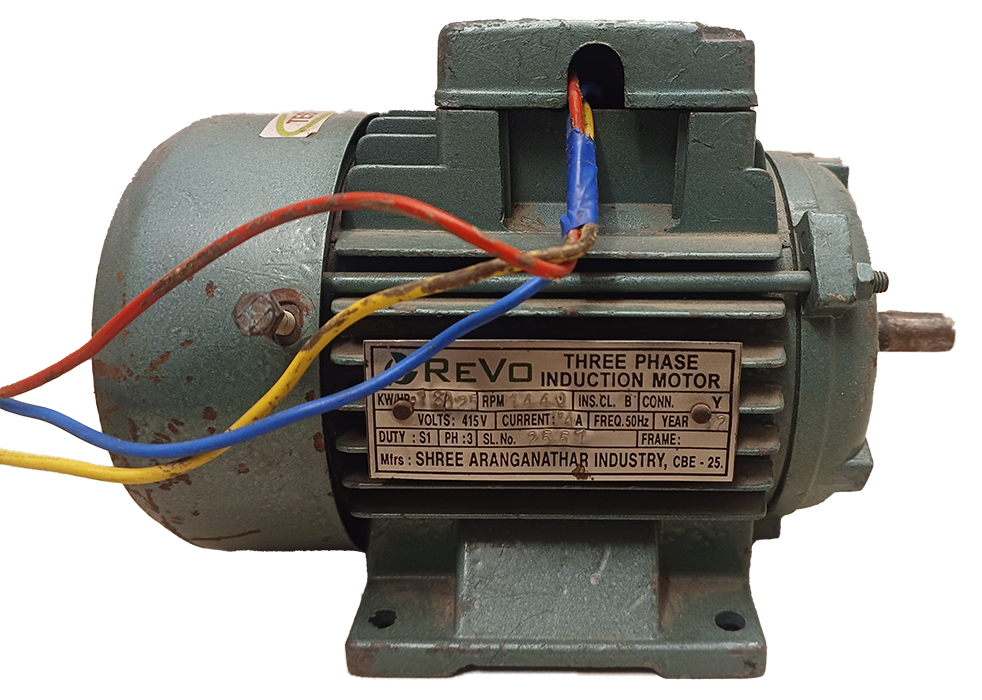
\includegraphics[width=3in]{sections/section4/images/inductionMotor/revo.png}}

		\caption{Induction Motor}

	\end{figure}
\end{frame}

\begin{frame}{Harware block diagram}
	\begin{figure}
		\centering

		\fbox{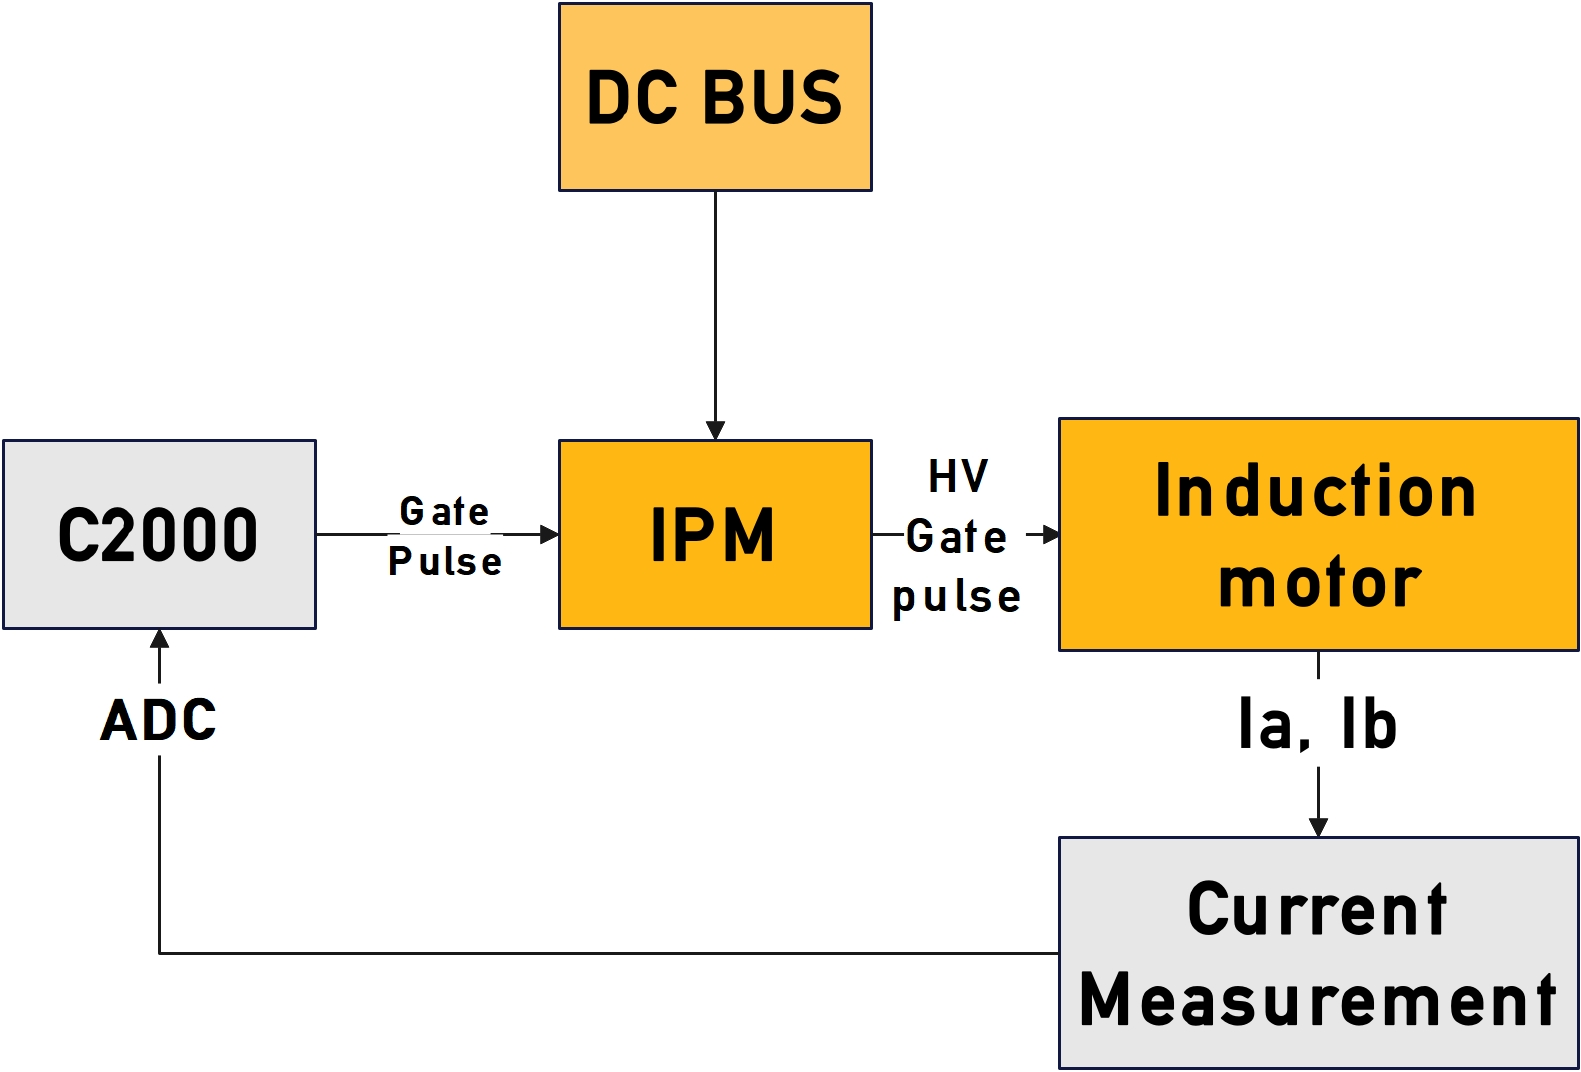
\includegraphics[width=4in]{sections/section4/images/SingleLineHardware.jpg}}

		\caption{Harware block diagram}
	\end{figure}
\end{frame}


\begin{frame}{ACIM Parameter Estimation: No-Load Test}
	\begin{columns}
	  \column{0.5\textwidth}
		\begin{figure}
		  \centering
		  \fbox{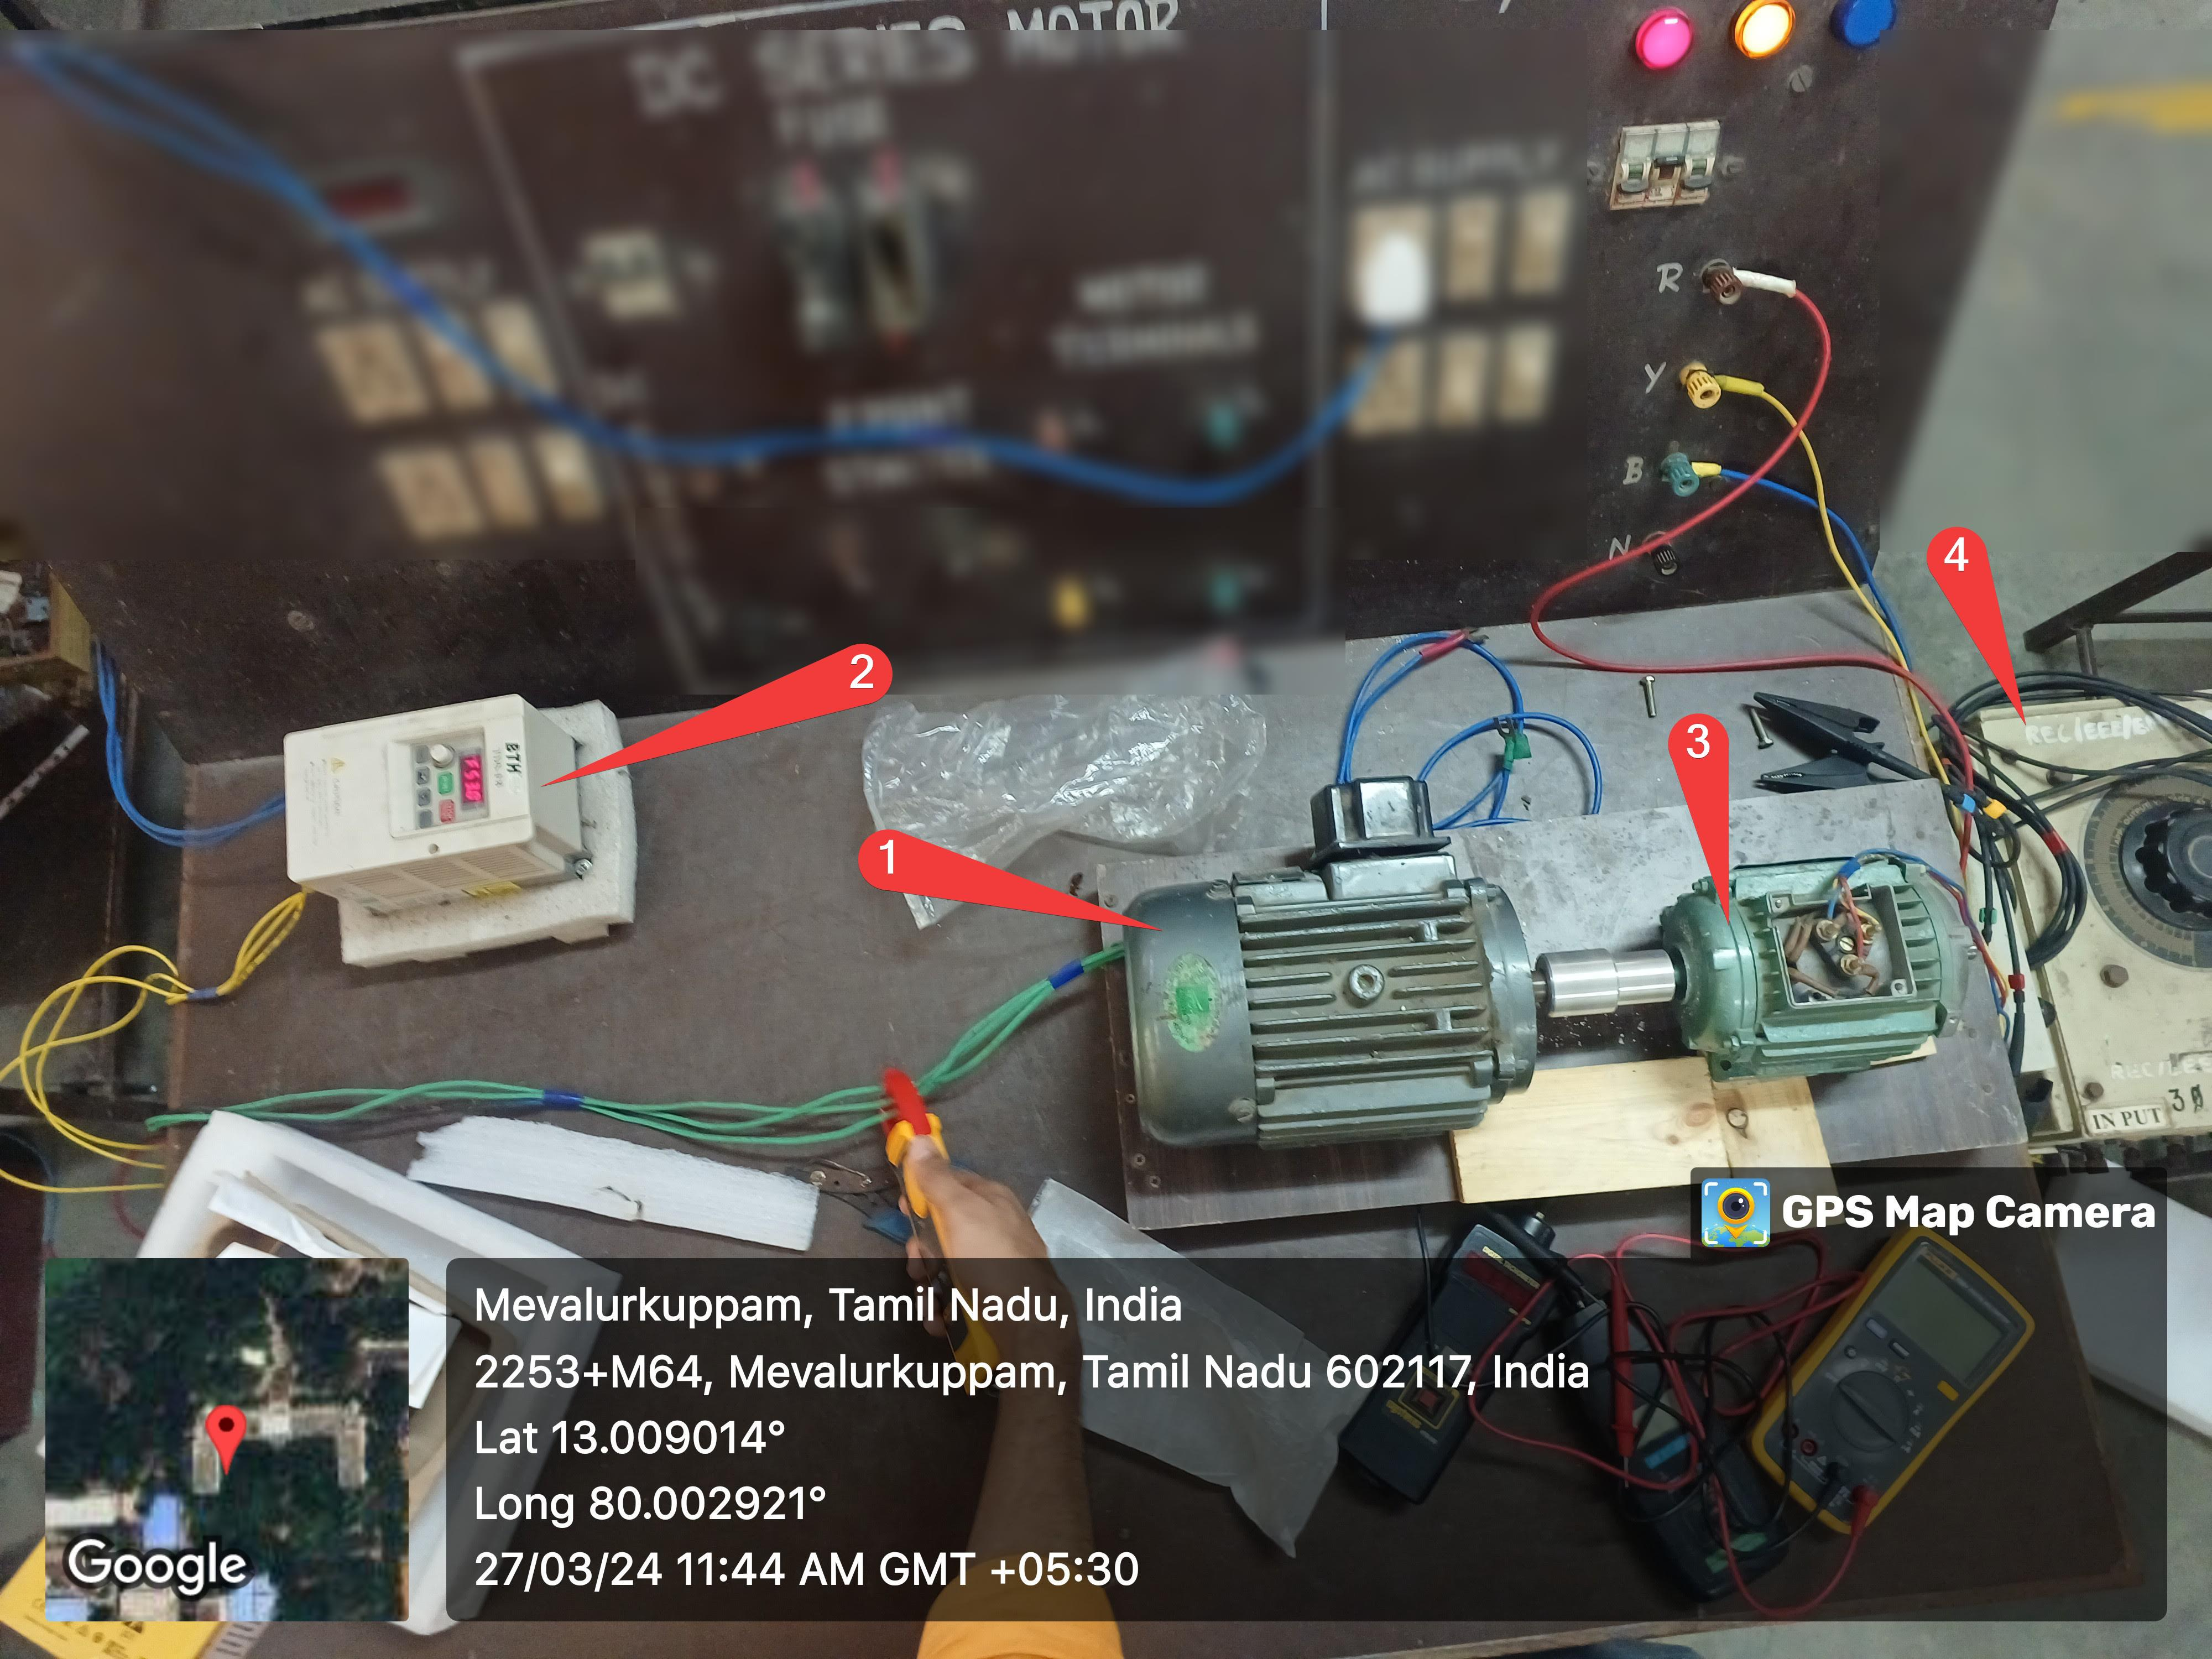
\includegraphics[width=2.2in]{sections/section5/images/ParamEstim/SetupNoload.jpg}}
		  \caption{No-load test setup}
		\end{figure}
		\begin{itemize}
		  \item Slip speed is made zero.
		\end{itemize}
	  \column{0.5\textwidth}
		\begin{figure}
		  \centering
		  \fbox{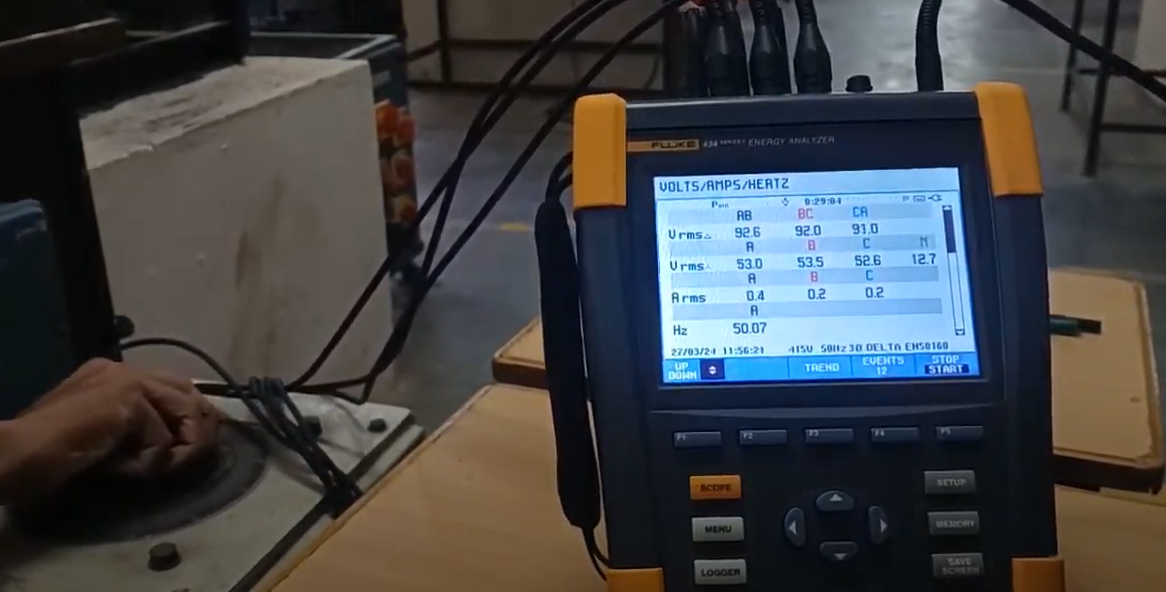
\includegraphics[width=2.2in]{sections/section5/images/ParamEstim/FlukeVoltAmpHertz.png}}
		  \caption{Fluke 434 power analyzer}
		\end{figure}
	\end{columns}
  \end{frame}

% Slide: No-load and Blocked Rotor Test Circuits
\begin{frame}{ACIM Parameter Estimation: Test Circuits}
	\begin{columns}
	  \column{0.5\textwidth}
		\begin{figure}
		  \centering
		  \fbox{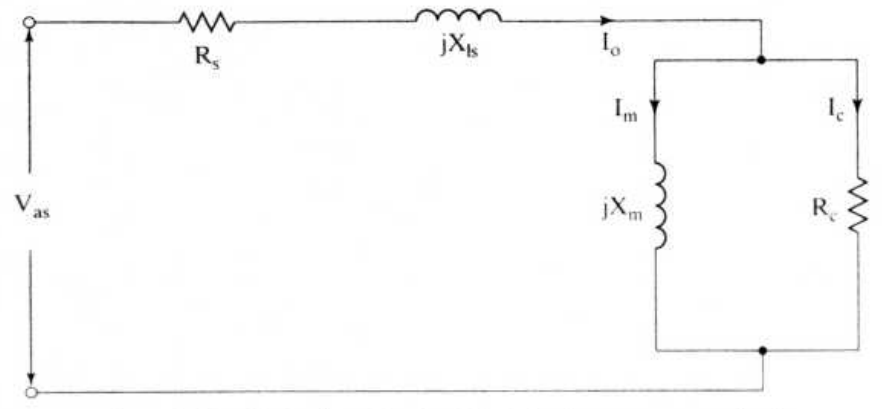
\includegraphics[width=2in]{sections/section5/images/ParamEstim/noloadCircuitKrish.png}}
		  \caption{No-load test circuit}
		\end{figure}
	  \column{0.5\textwidth}
		\begin{figure}
		  \centering
		  \fbox{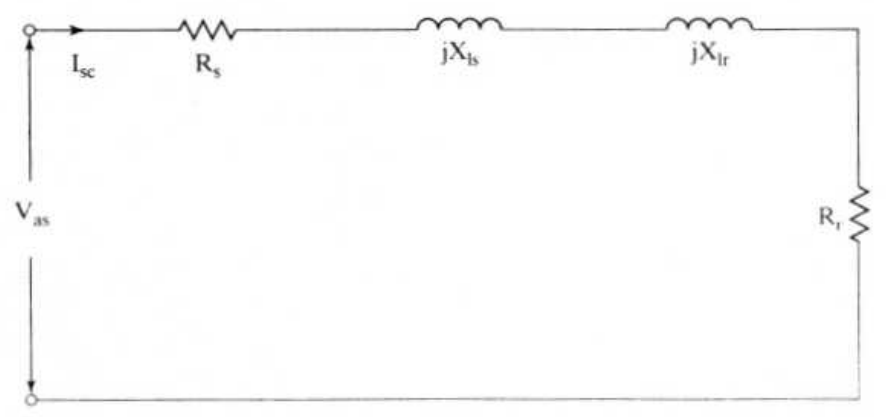
\includegraphics[width=2in]{sections/section5/images/ParamEstim/blockedCircuitKrish.png}}
		  \caption{Blocked rotor test circuit}
		\end{figure}
	\end{columns}
  \end{frame}
% ACIM formuls

\begin{frame}{ACIM Parameter Estimation Formulas}
	\begin{columns}[T] % Align columns at the top

		\begin{column}{0.48\textwidth} % Adjust column widths as needed

			\textbf{No-Load Test:}

			\begin{align*}
				\cos \phi_0 & = \frac{P_i}{V_\text{as}I_0}             \\
				I_m         & = I_0 \sin \phi_0                        \\
				I_c         & = I_0 \cos \phi_0                        \\
				L_m         & = \frac{V_\text{as}}{2\pi f_\text{i}I_m} \\
				R_c         & = \frac{V_\text{as}}{I_c}
			\end{align*}

		\end{column}

		\begin{column}{0.48\textwidth}

			\textbf{Blocked Rotor Test:}

			\begin{align*}
				\cos \phi_\text{sc} & = \frac{P_\text{sc}}{V_\text{sc}I_\text{sc}} \\
				Z_\text{sc}         & = \frac{V_\text{sc}}{I_\text{sc}}            \\
				R_r                 & = Z_\text{sc} \cos \phi_\text{sc} - R_s      \\
				X_\text{eq}         & = Z_\text{sc} \sin \phi_\text{sc}            \\
				X_\text{eq}         & = X_\text{ls} + X_\text{lr}
			\end{align*}

		\end{column}

	\end{columns}
\end{frame}


% ACIM parameter estimation results excel sheet image

\begin{frame}{ACIM Parameter Estimation Results}
	\begin{figure}
		\centering

		\fbox{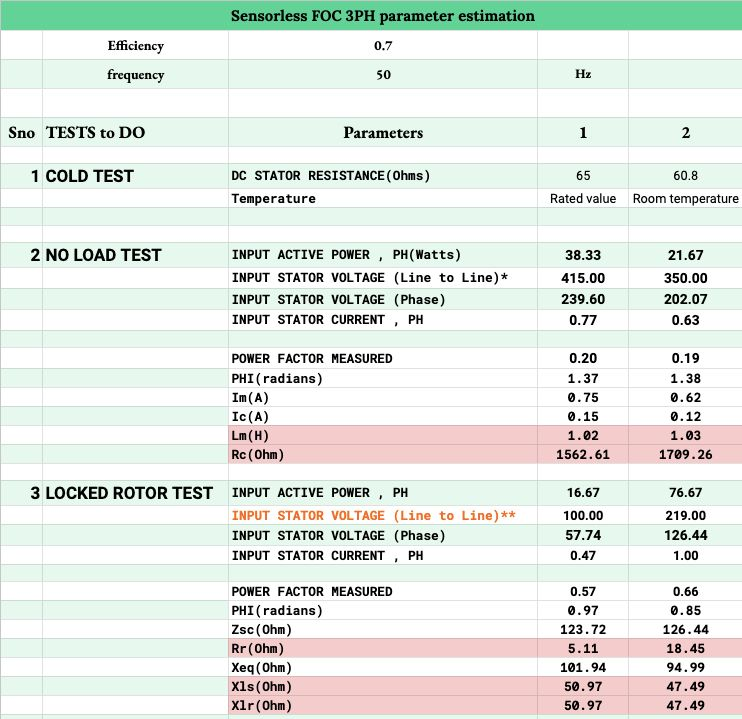
\includegraphics[width=2.8in]{sections/ppt/acim.jpg}}

		\caption{ACIM Parameter Estimation Results}
	\end{figure}
\end{frame}





\begin{frame}{PCB Design}
	\begin{figure}
		\centering

		\fbox{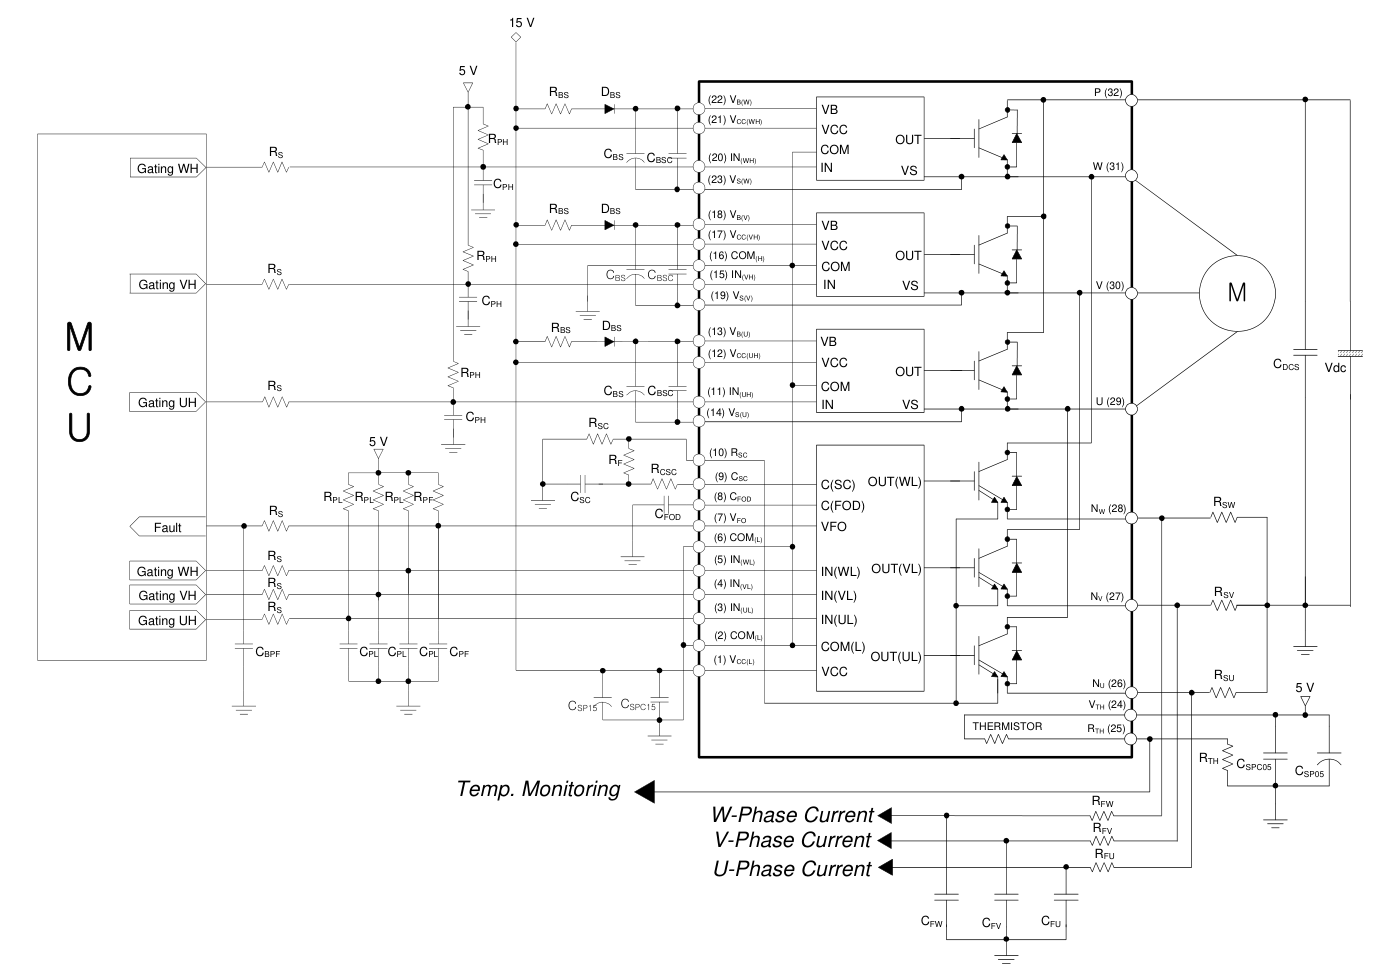
\includegraphics[width=4in]{sections/section4/images/PCBDesign/ApplicationCircuitfromDatasheet.png}}

	\end{figure}
\end{frame}


% MCU interface circuit

\begin{frame}{MCU Interface Circuit}
	\begin{figure}
		\centering

		\fbox{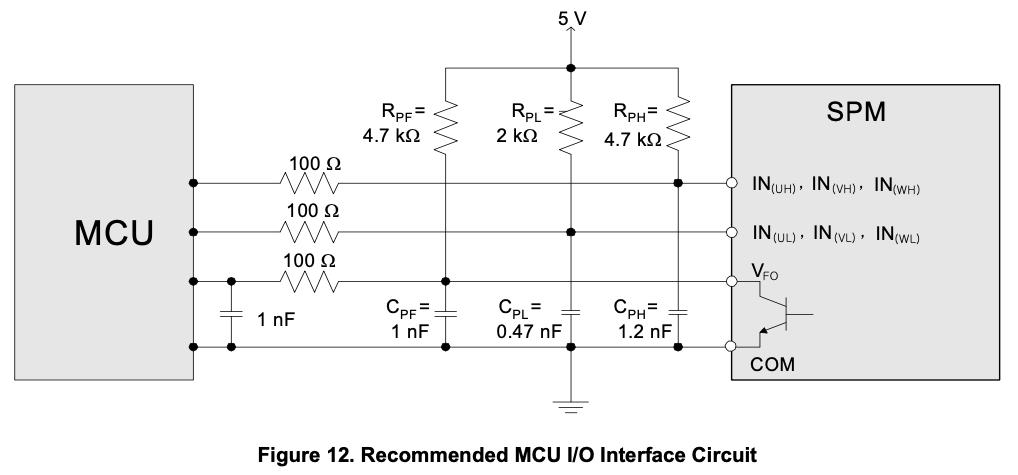
\includegraphics[width=4in]{sections/ppt/mcuInt.jpg}}

		\caption{MCU Interface Circuit}
	\end{figure}

	\begin{itemize}
		\item Bypass capacitors ground H.F. oscillations, decoupling DC circuit from A.C. Noise.
		\item Input pullup removes load strain on MCU.
	\end{itemize}
\end{frame}


% Short circuit protection circuit image

\begin{frame}{Short Circuit Protection Circuit}
	\begin{figure}
		\centering

		\fbox{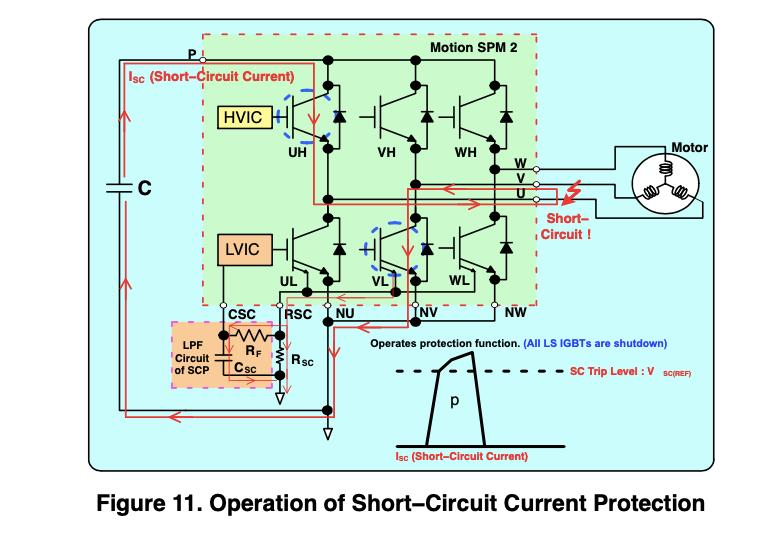
\includegraphics[width=2.8in]{sections/ppt/short-circuit-protection.jpg}}

		\caption{Short Circuit Protection Circuit}
	\end{figure}


	\begin{itemize}
		\item Seperate open-emitter pins are provided from low-side IGBTs for current sensing.
	\end{itemize}
\end{frame}



% Under voltage lockout circuit image

\begin{frame}{Under Voltage Lockout Circuit}
	\begin{figure}
		\centering

		\fbox{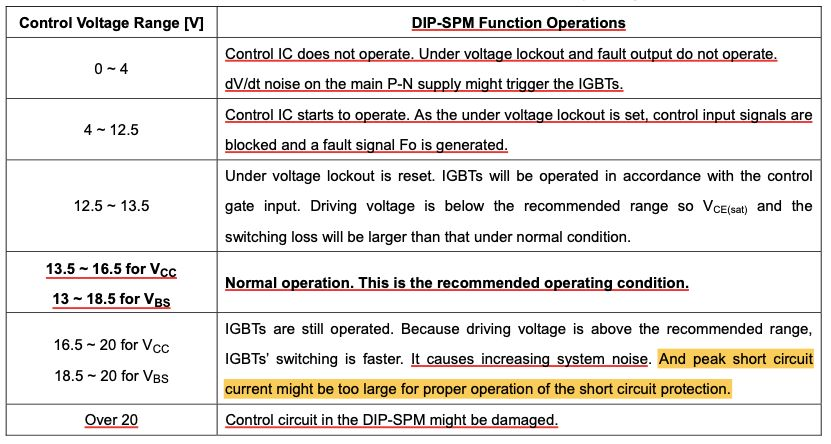
\includegraphics[width=4in]{sections/ppt/UVLC.jpg}}

		\caption{Under Voltage Lockout Circuit}
	\end{figure}
\end{frame}

% Bootstaro circyut image

\begin{frame}{Bootstrap Circuit}
	\begin{figure}
		\centering

		\fbox{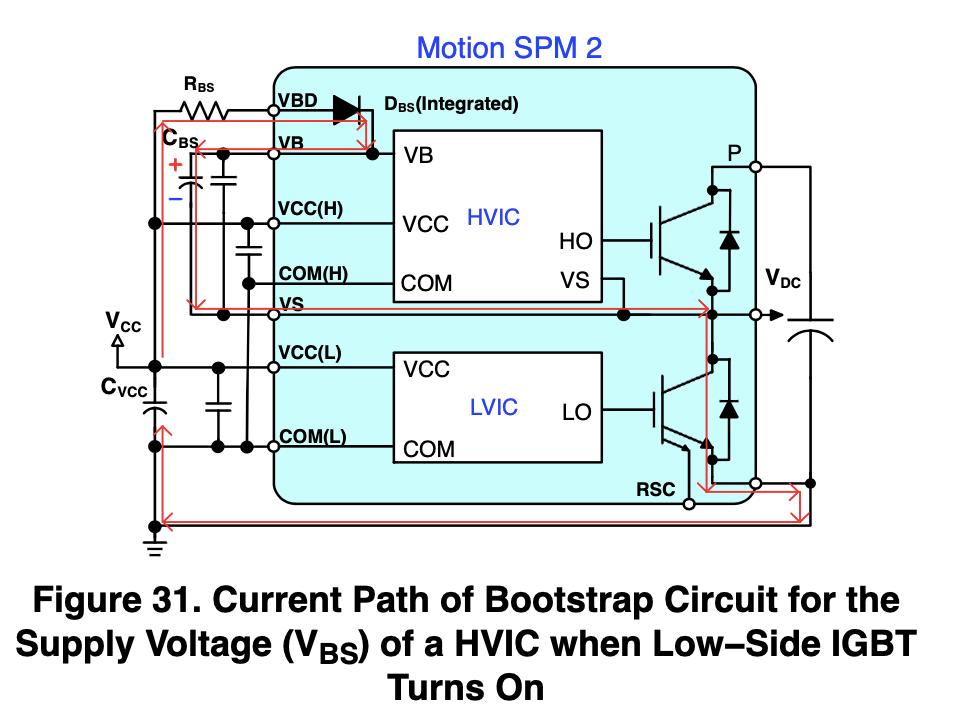
\includegraphics[width=2.8in]{sections/ppt/bootstrap.jpg}}

		\caption{Bootstrap Circuit}
	\end{figure}

	\begin{itemize}
		\item Charges when low-side switch is on and supplies 15V across high side IGBT gate-emitter
	\end{itemize}
\end{frame}


% Bootstrap intial charging formula image

\begin{frame}{Bootstrap Initial Charging}
	\begin{figure}
		\centering

		\fbox{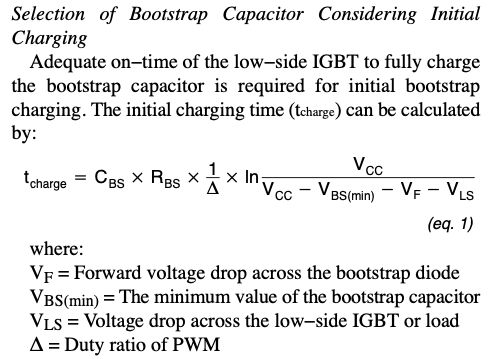
\includegraphics[width=4in]{sections/ppt/initalCharging.jpg}}

		\caption{Bootstrap Initial Charging}
	\end{figure}
\end{frame}

% Bootstrap intial charging  graph image

\begin{frame}{Bootstrap Initial Charging}
	\begin{figure}
		\centering

		\fbox{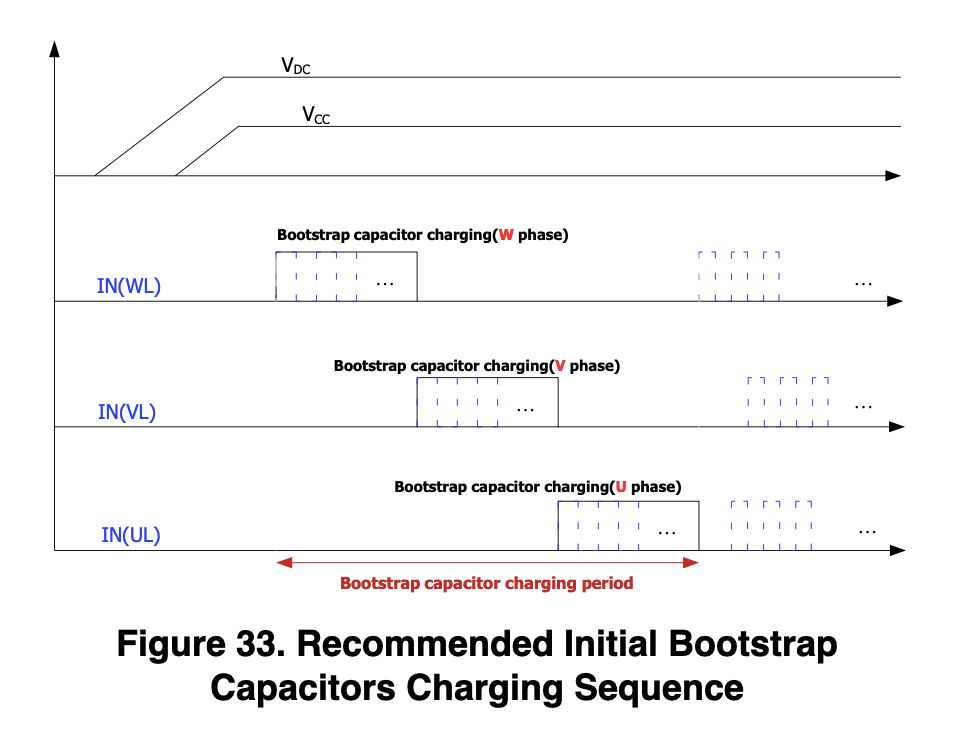
\includegraphics[width=3.5in]{sections/ppt/initalChargingGraph.jpg}}

		\caption{Bootstrap Initial Charging}
	\end{figure}
\end{frame}

% Slide 19: PCB Layout Design in Ultiboard
\begin{frame}{PCB Layout Design}
	\begin{figure}
		\centering

		\fbox{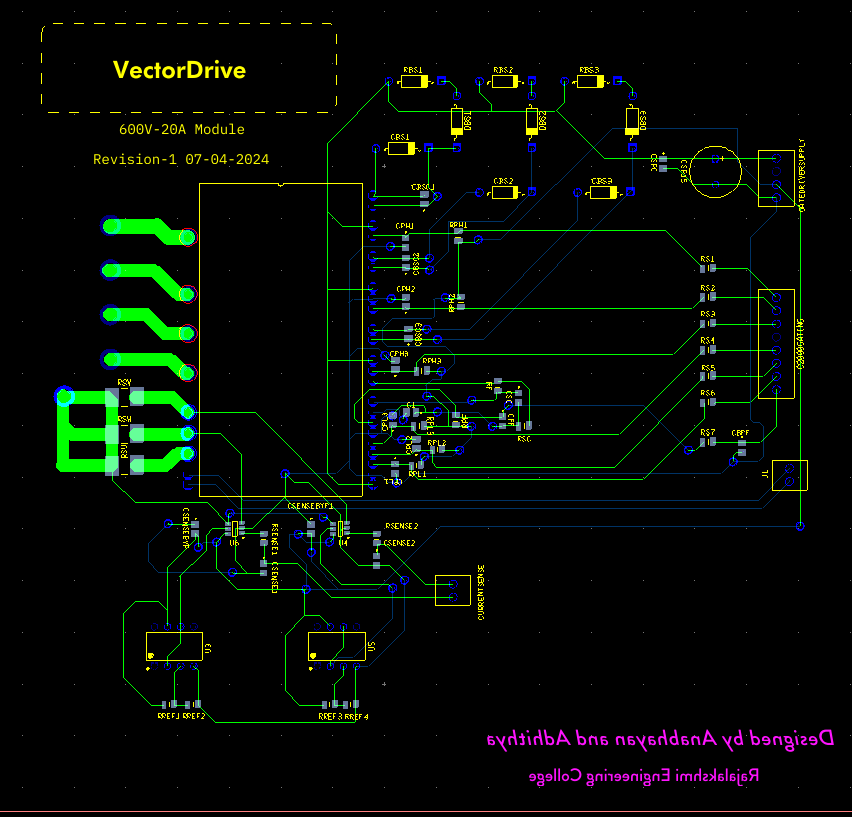
\includegraphics[width=2.5in]{sections/section4/images/PCBDesign/Ultiboard/Ultiboard.png}}

		\caption{PCB Layout Design in Ultiboard}
	\end{figure}
\end{frame}

% Slide 20: 3D View of PCB Layout Design in Ultiboard
\begin{frame}{3D View of PCB Layout}
	\begin{figure}
		\centering

		\fbox{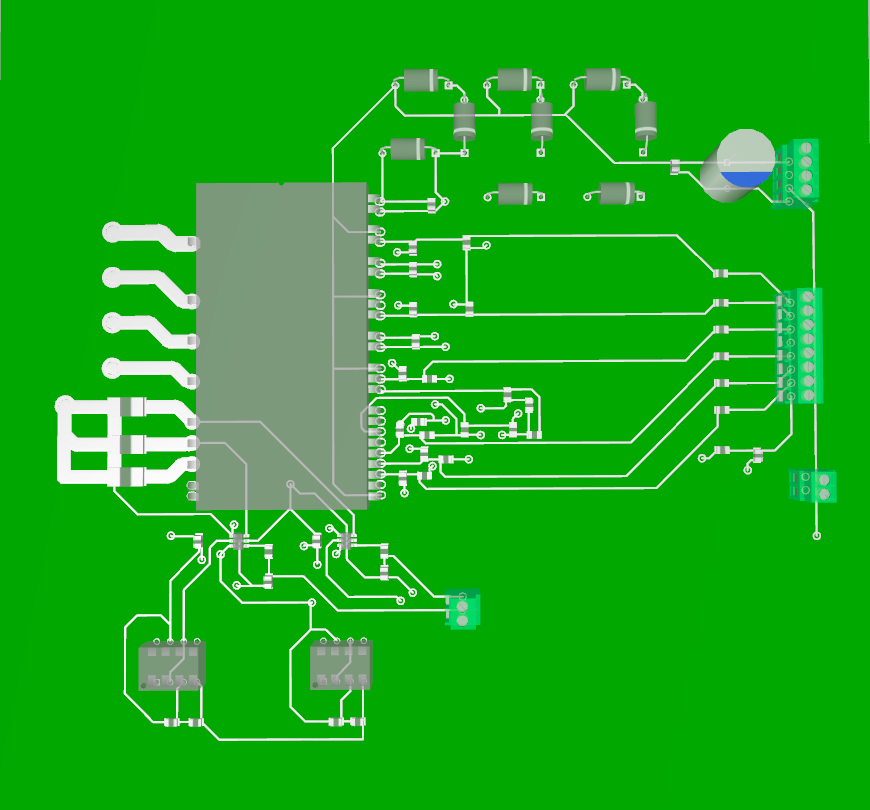
\includegraphics[width=2.5in]{sections/section4/images/PCBDesign/Ultiboard/3DTopView.png}}

		\caption{3D View of PCB Layout Design in Ultiboard}

	\end{figure}
\end{frame}


% Current sense circuit image block diagram

\begin{frame}{Current Sensing Circuit}
	\begin{figure}
		\centering

		\fbox{\includegraphics[width=2.8in]{sections/ppt/currentSense.jpg}}

		\caption{Current Sensing Circuit}
	\end{figure}


	\begin{itemize}
		\item Differential amplifier is connected across shunt resistor and postive side DC shifted by $V_{cc}\over 2$ for bi-directional current sensing.
	\end{itemize}
\end{frame}

% Slide 21: Current Sensing Circuit in Multisim
\begin{frame}{Current Measurement}
	\begin{figure}
		\centering

		\fbox{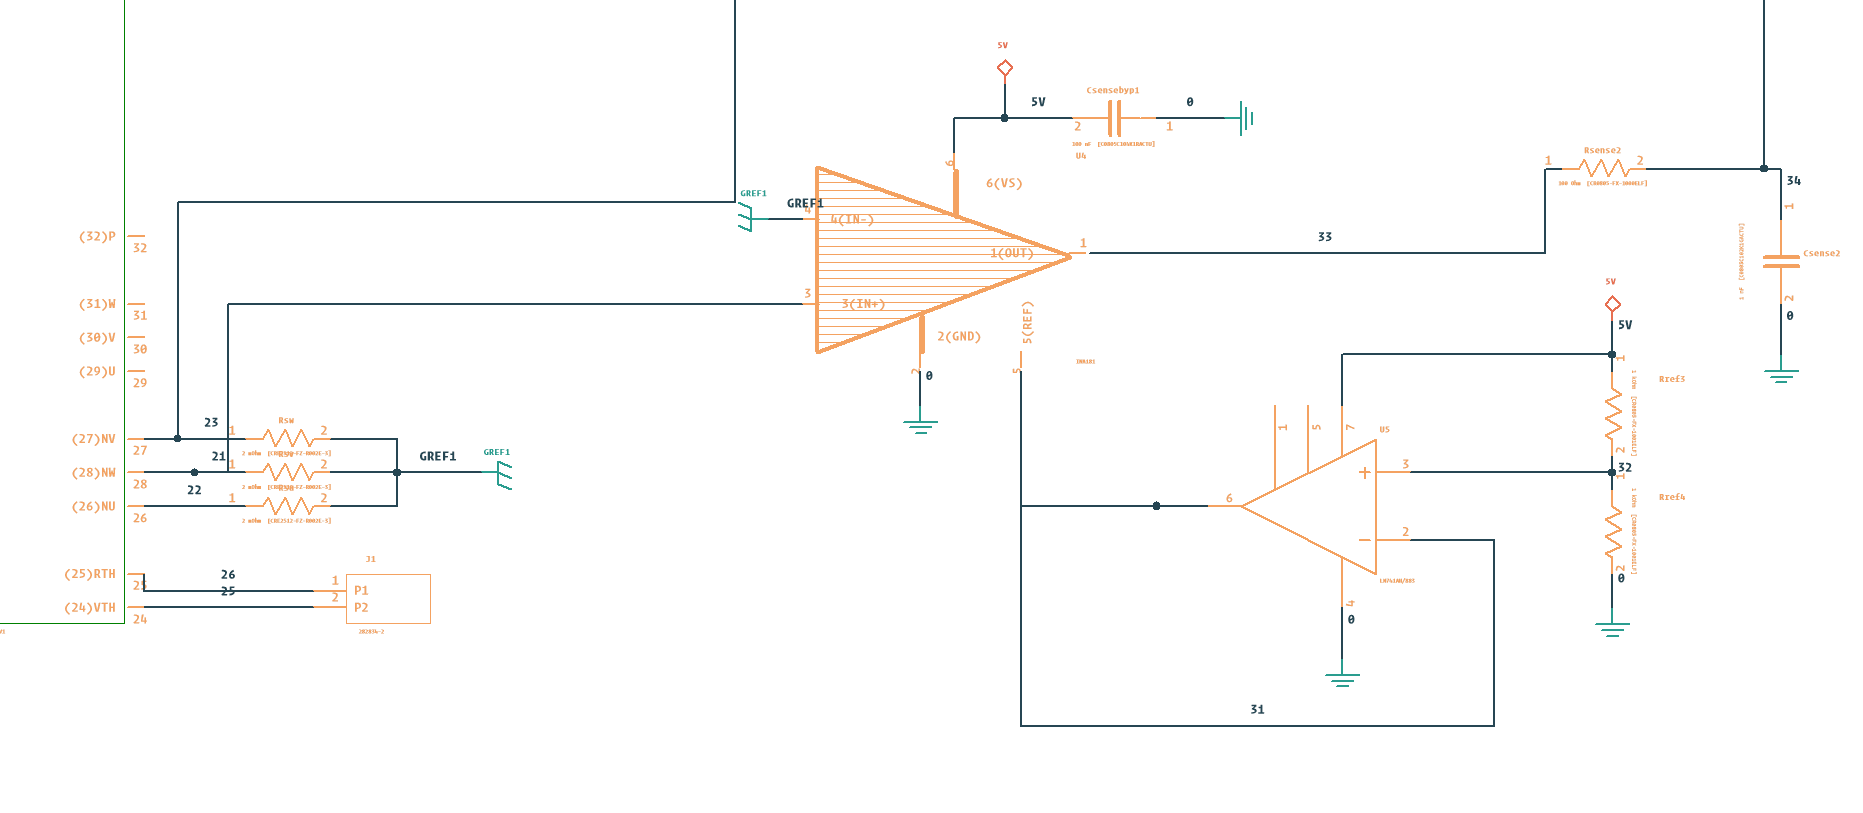
\includegraphics[width=4in]{sections/section4/images/PCBDesign/Multisim/MultisimCurrentSensing.png}}

		\caption{Current Sensing Circuit in Multisim (one phase shown)}
	\end{figure}
\end{frame}

% ePWM module block diagram

\begin{frame}{ePWM Module}
	\begin{figure}
		\centering

		\fbox{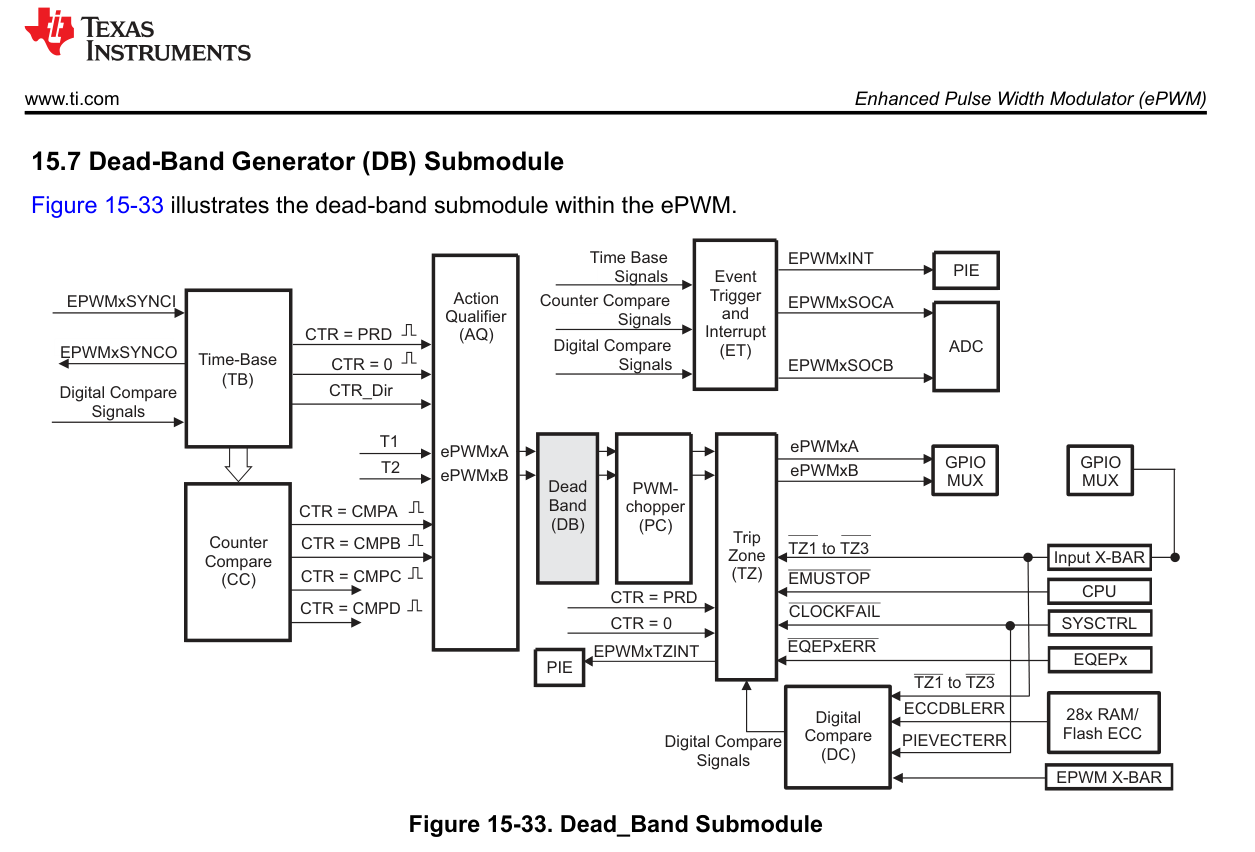
\includegraphics[width=4in]{sections/ppt/ePWM.png}}

		\caption{ePWM Module}
	\end{figure}
\end{frame}

% Slide 26: ePWM block in Simulink
\begin{frame}{Space Vector Pulse Width Modulation}
	\begin{figure}
		\centering

		\fbox{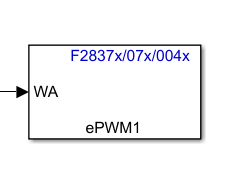
\includegraphics[width=2in]{sections/section6/images/SVPWM/ePWMBlock.png}}

		\caption{ePWM block in Simulink}
	\end{figure}
\end{frame}


% Counter compare and timer period visualtion 1

\begin{frame}{Counter Compare and Timer Period Visualization}
	\begin{figure}
		\centering
		\fbox{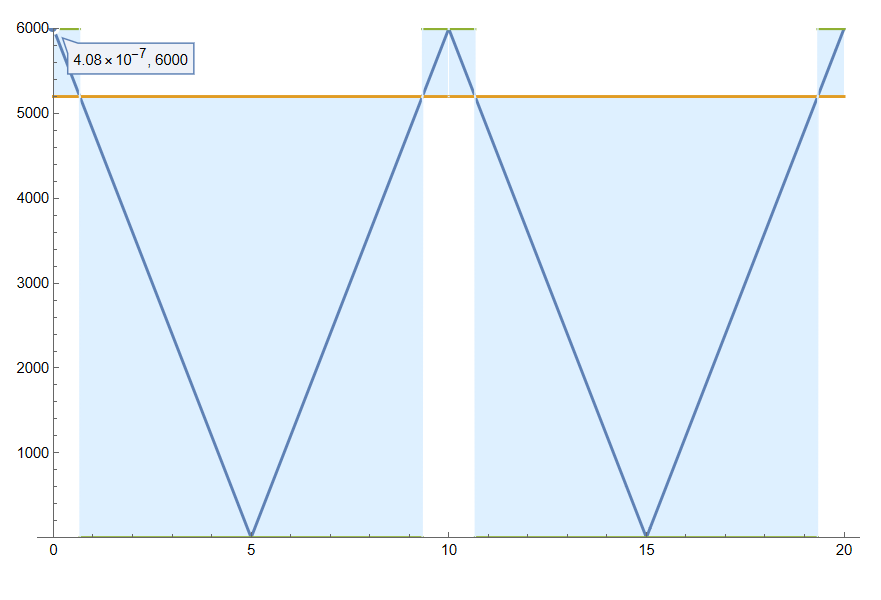
\includegraphics[width=4in]{sections/ppt/CC1.png}}
		\caption{Counter Compare High}
	\end{figure}
\end{frame}

\begin{frame}{Counter Compare and Timer Period Visualization}
	\begin{figure}
		\centering
		\fbox{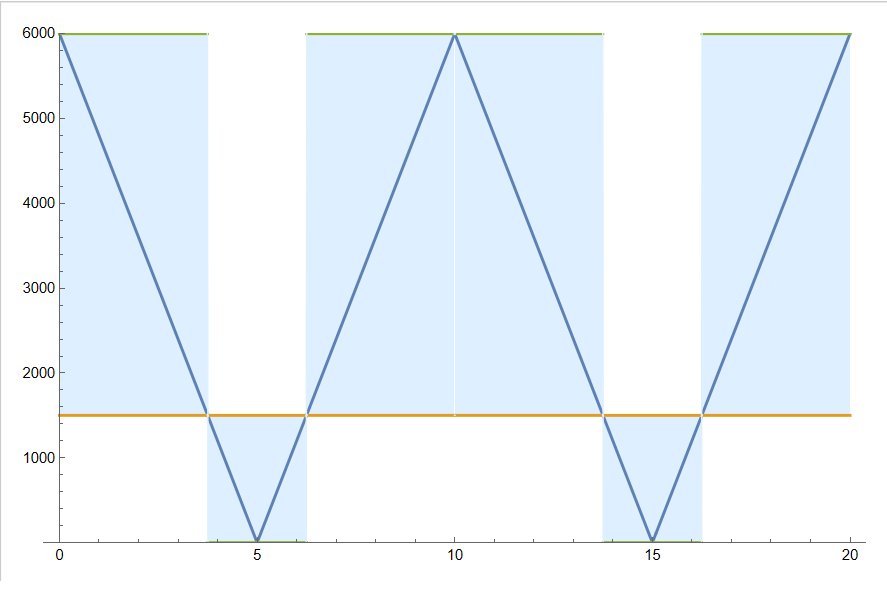
\includegraphics[width=4in]{sections/ppt/CC2.png}}
		\caption{Counter Compare Low}
	\end{figure}
\end{frame}

\begin{frame}{Counter Compare and Timer Period Visualization}
	\begin{figure}
		\centering
		\fbox{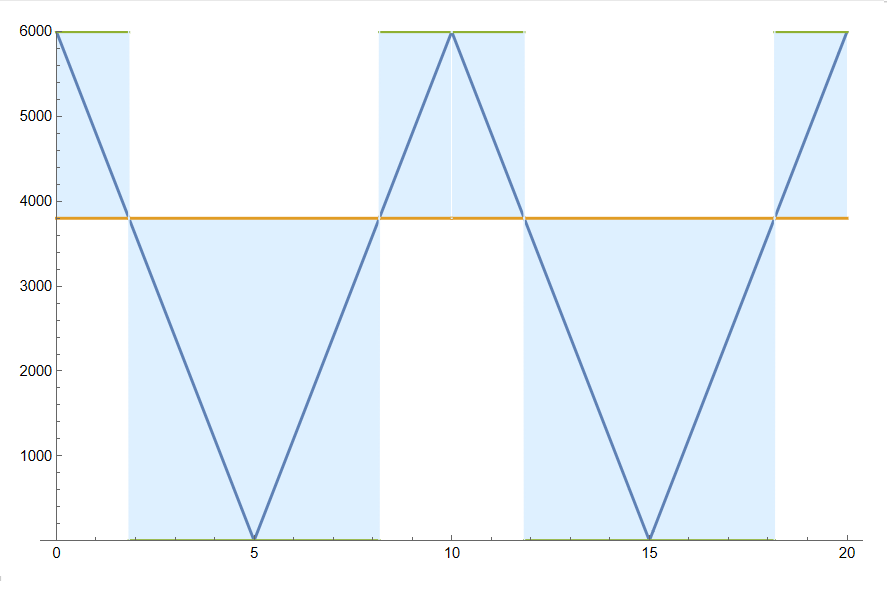
\includegraphics[width=4in]{sections/ppt/CC3.png}}
		\caption{Counter Compare half}
	\end{figure}
\end{frame}


\begin{frame}{TBPRD Calculation}

	\begin{columns}[T]
		\column{0.5\textwidth}
		\begin{itemize}
			\item PWM Frequency ($F_{PWM}$): 15 kHz (recommended by FSAM20SH60A datasheet)
			\item System Clock (SYSCLK): 200 MHz
			\item High Speed Clock Divider (HSPCLKDIV): 1
			\item Clock Divider (CLKDIV): 1
		\end{itemize}
		\column{0.5\textwidth}
		\begin{align*}
			T_{PWM}   & = \frac{1}{F_{PWM}}                      \\
			T_{TBCLK} & = \frac{SYSCLK}{HSPCLKDIV \times CLKDIV} \\
			TBPRD     & = \frac{T_{PWM}}{2 \times T_{TBCLK}}
		\end{align*}
	\end{columns}

	\vspace{0.5cm}

	\begin{align*}
		T_{PWM}   & = \frac{1}{15 \times 10^3} \text{ seconds}                               \\
		T_{TBCLK} & = \frac{200 \times 10^6}{1 \times 1} = 200 \times 10^6 \text{ Hz}        \\
		TBPRD     & = \frac{\frac{1}{15 \times 10^3}}{2 \times 200 \times 10^6} \approx 6667
	\end{align*}

	\tiny{Therefore, the Timer Period (TBPRD) is 6667.}
\end{frame}


\begin{frame}{ePWM Configuration}
	\begin{figure}
		\centering
		\fbox{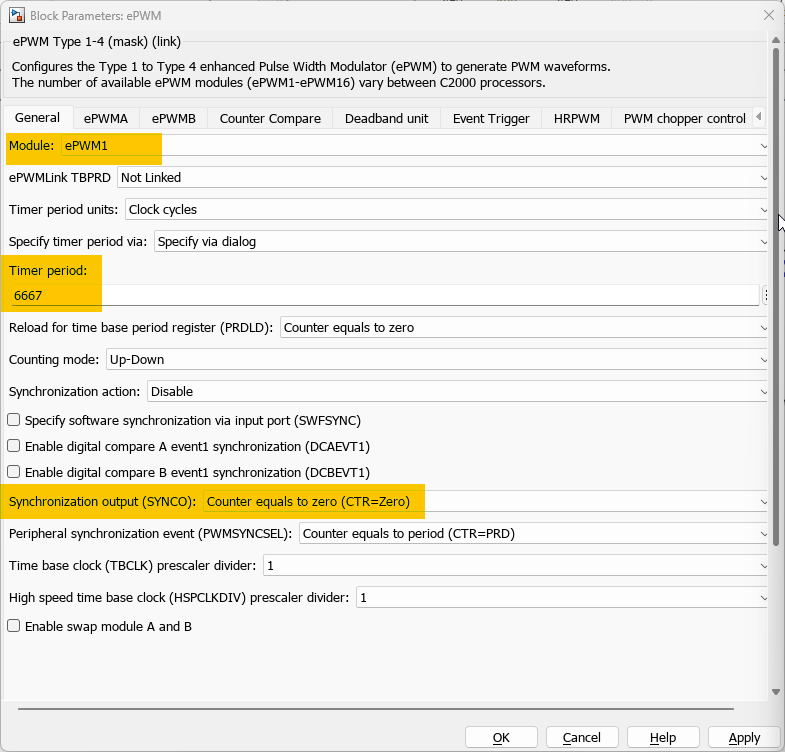
\includegraphics[width=3in]{sections/section6/images/SVPWM/ePWMTBPRD.png}}
		\caption{ePWM configuration in Simulink}
	\end{figure}
\end{frame}


\begin{frame}{Space Vector Pulse Width Modulation (SVPWM)}

	\begin{figure}
		\centering
		\fbox{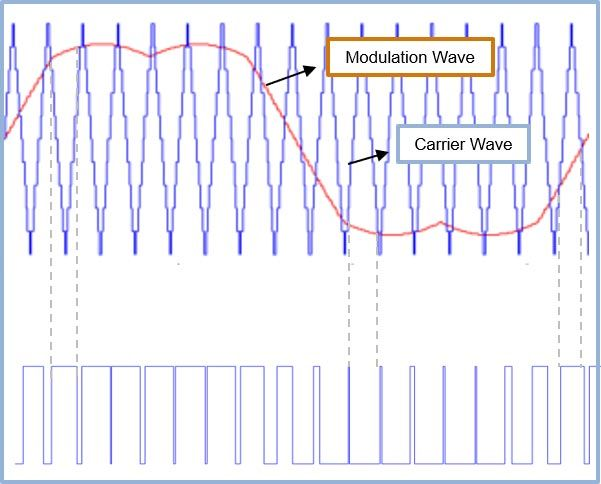
\includegraphics[width=2.2in]{sections/finalReview/svpwm.jpg}}
		\caption{Gate pulse generation}
	\end{figure}

	\begin{itemize}
		\item \textbf{Increased Efficiency:} SVPWM reduces harmonic distortion.
		\item \textbf{Higher Voltage Utilization:} SVPWM allows 15\% more DC bus voltage.
		\item \textbf{Reduced Switching Losses}
	\end{itemize}	

\end{frame}



\begin{frame}{Open loop: SVPWM}
	\begin{figure}
		\centering
		\fbox{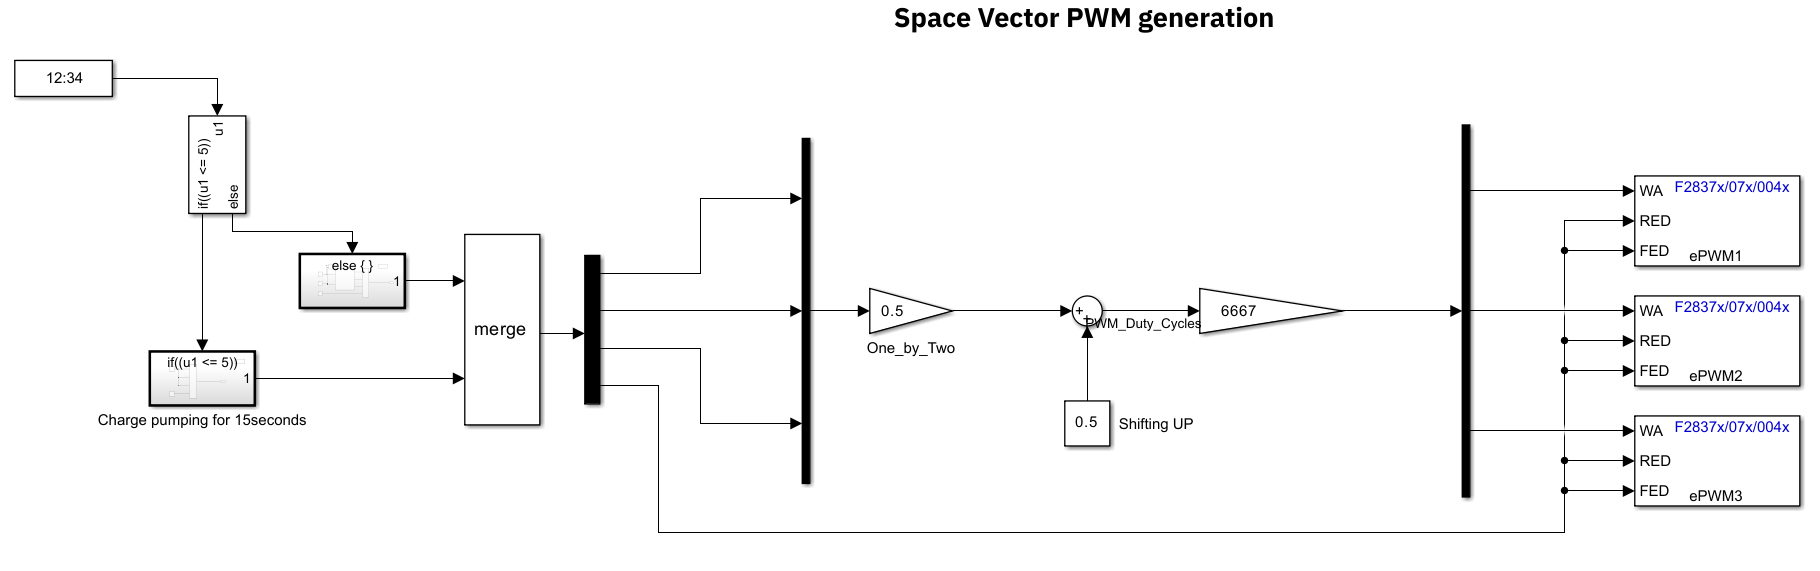
\includegraphics[width=4in]{sections/ppt/SVPWM_Simulink.png}}
		\caption{SVPWM Simulink Model}
	\end{figure}
\end{frame}


% Slide 28: Hardware setup with RC filter and Launchpad
\begin{frame}{SVPWM with Low Pass Filter}
	\begin{figure}
		\centering

		\fbox{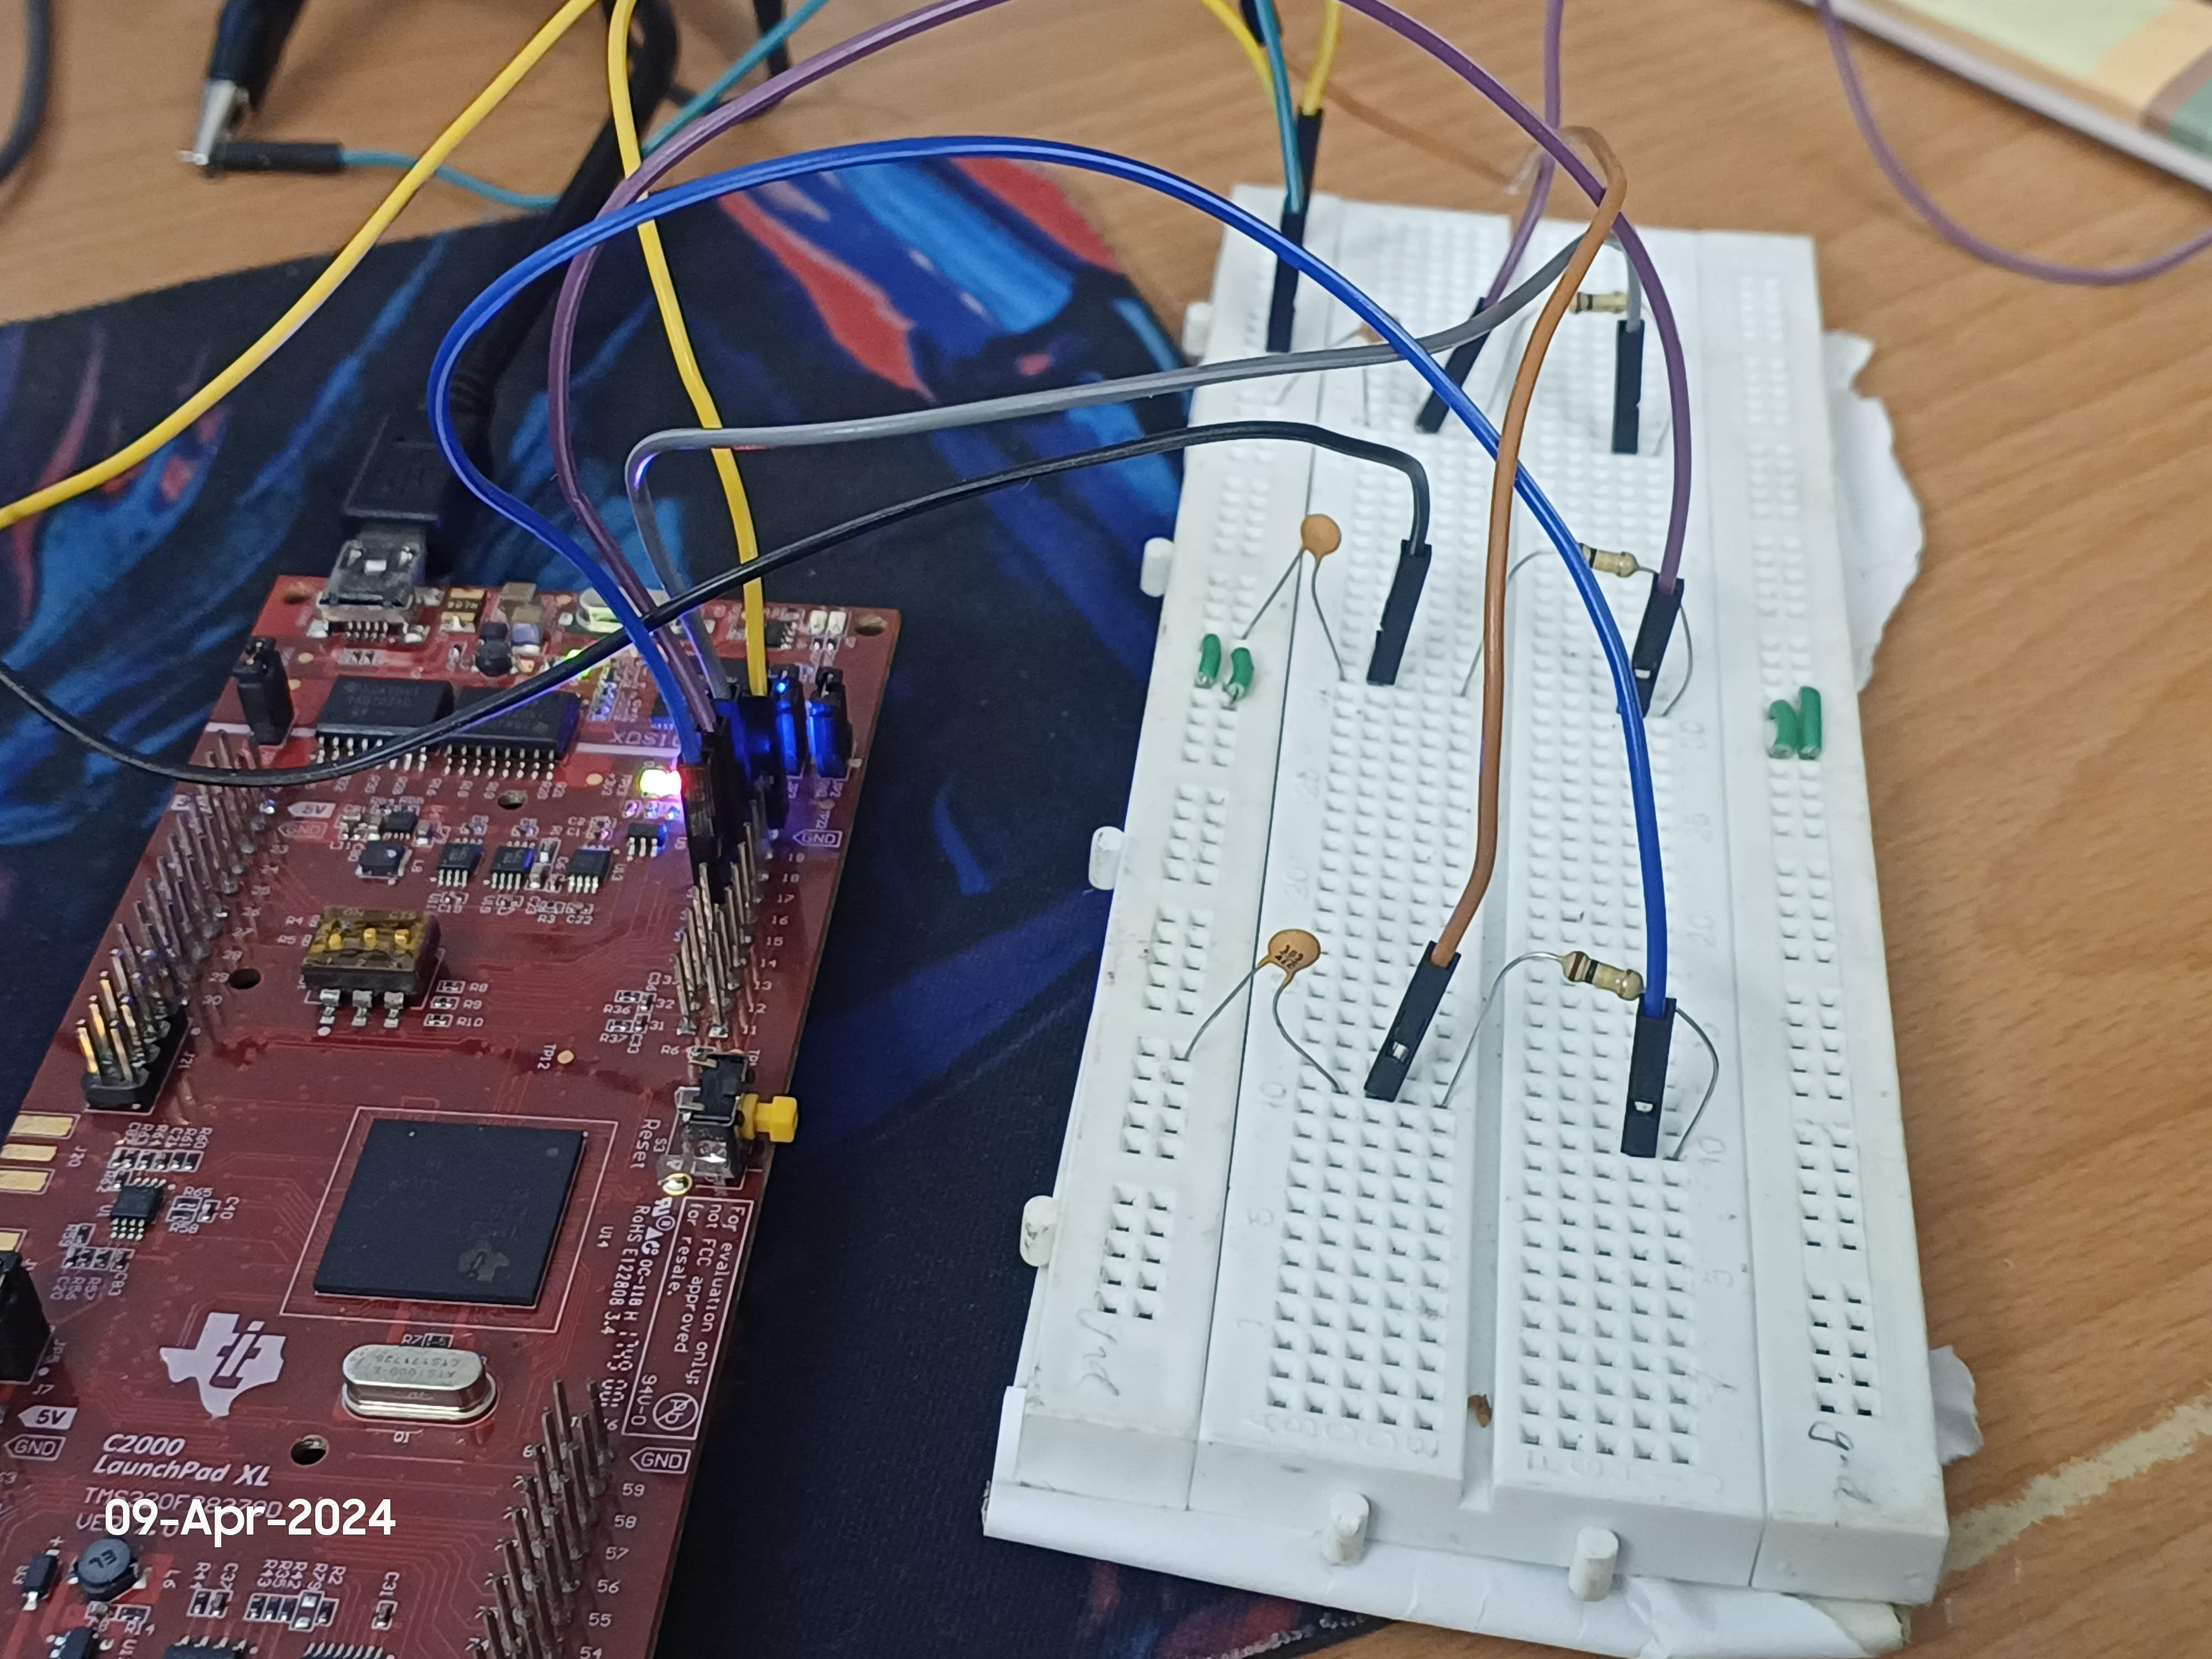
\includegraphics[width=4in]{sections/section6/images/SVPWM/LPFandC2000.jpg}}

		\caption{Hardware setup with RC filter and Launchpad}
	\end{figure}
\end{frame}

% Slide 29: Output of SVPWM with low pass filter
\begin{frame}{Output of SVPWM with LPF}
	\begin{figure}
		\centering

		\fbox{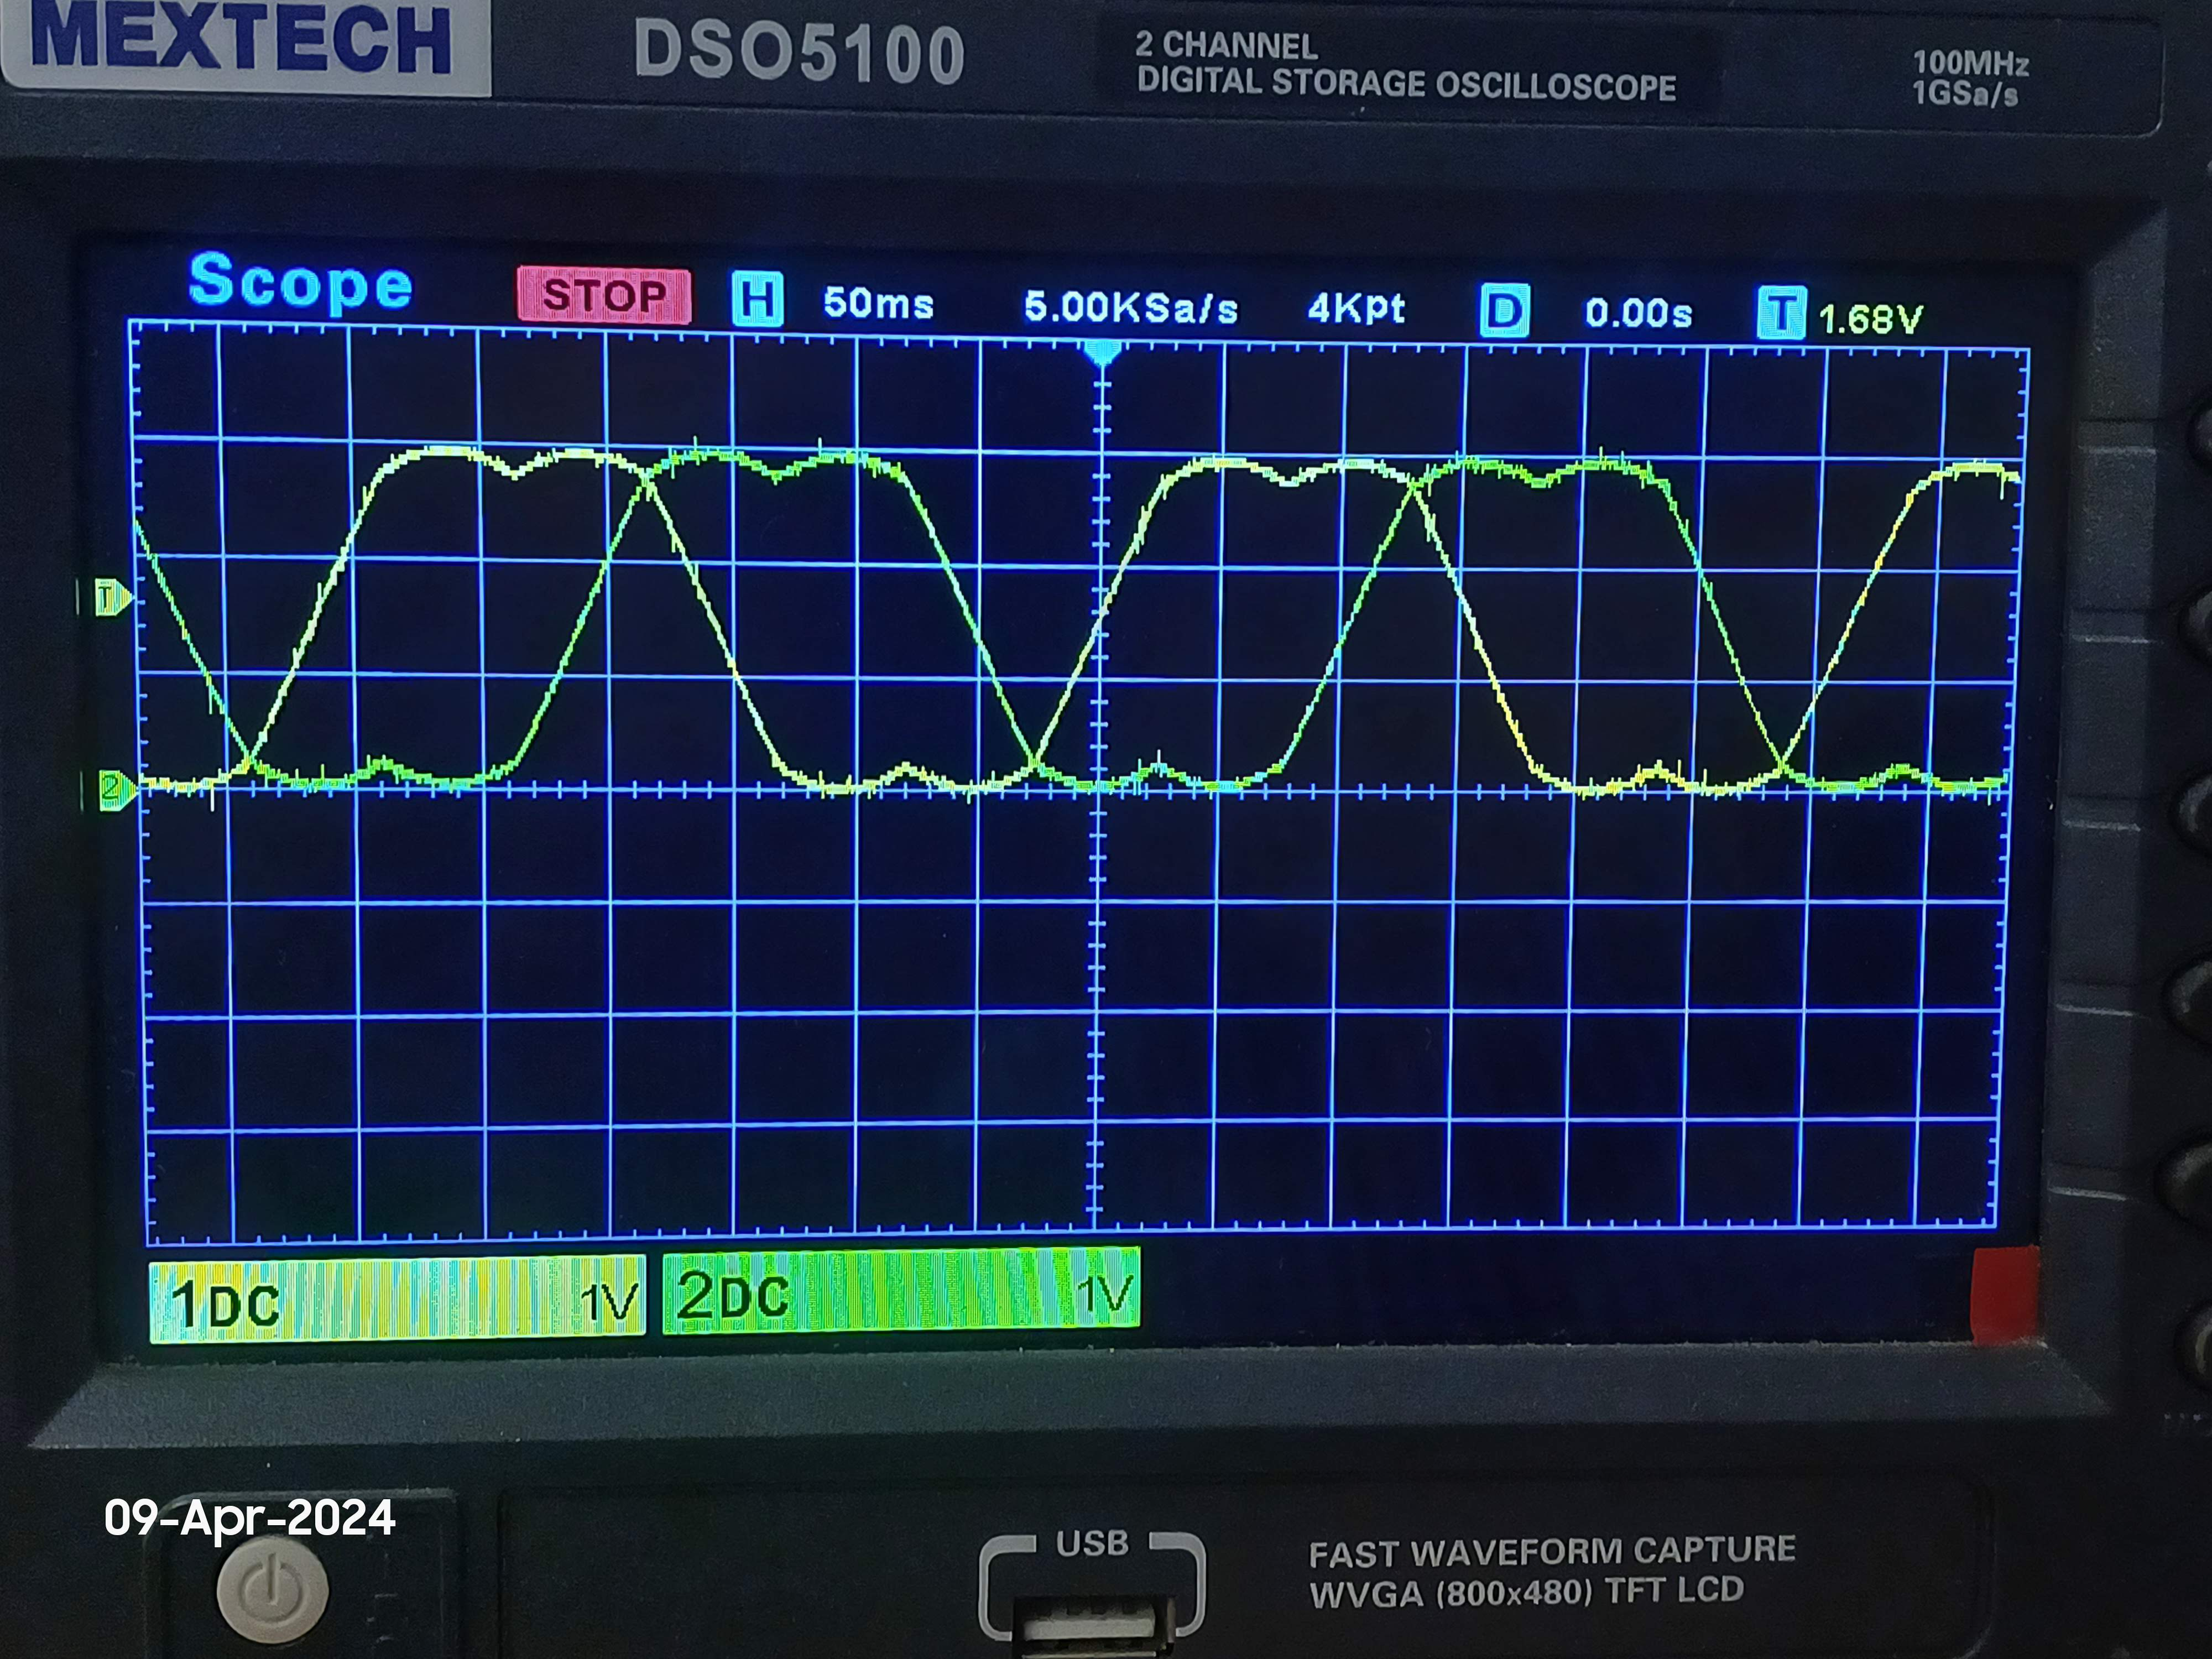
\includegraphics[width=4in]{sections/section6/images/SVPWM/SVPWM2phases.jpg}}

		\caption{Output of SVPWM with low pass filter}
	\end{figure}
\end{frame}


% Slide 30: Dead band time
\begin{frame}{Dead Band Configuration}
	\begin{figure}
		\centering

		\fbox{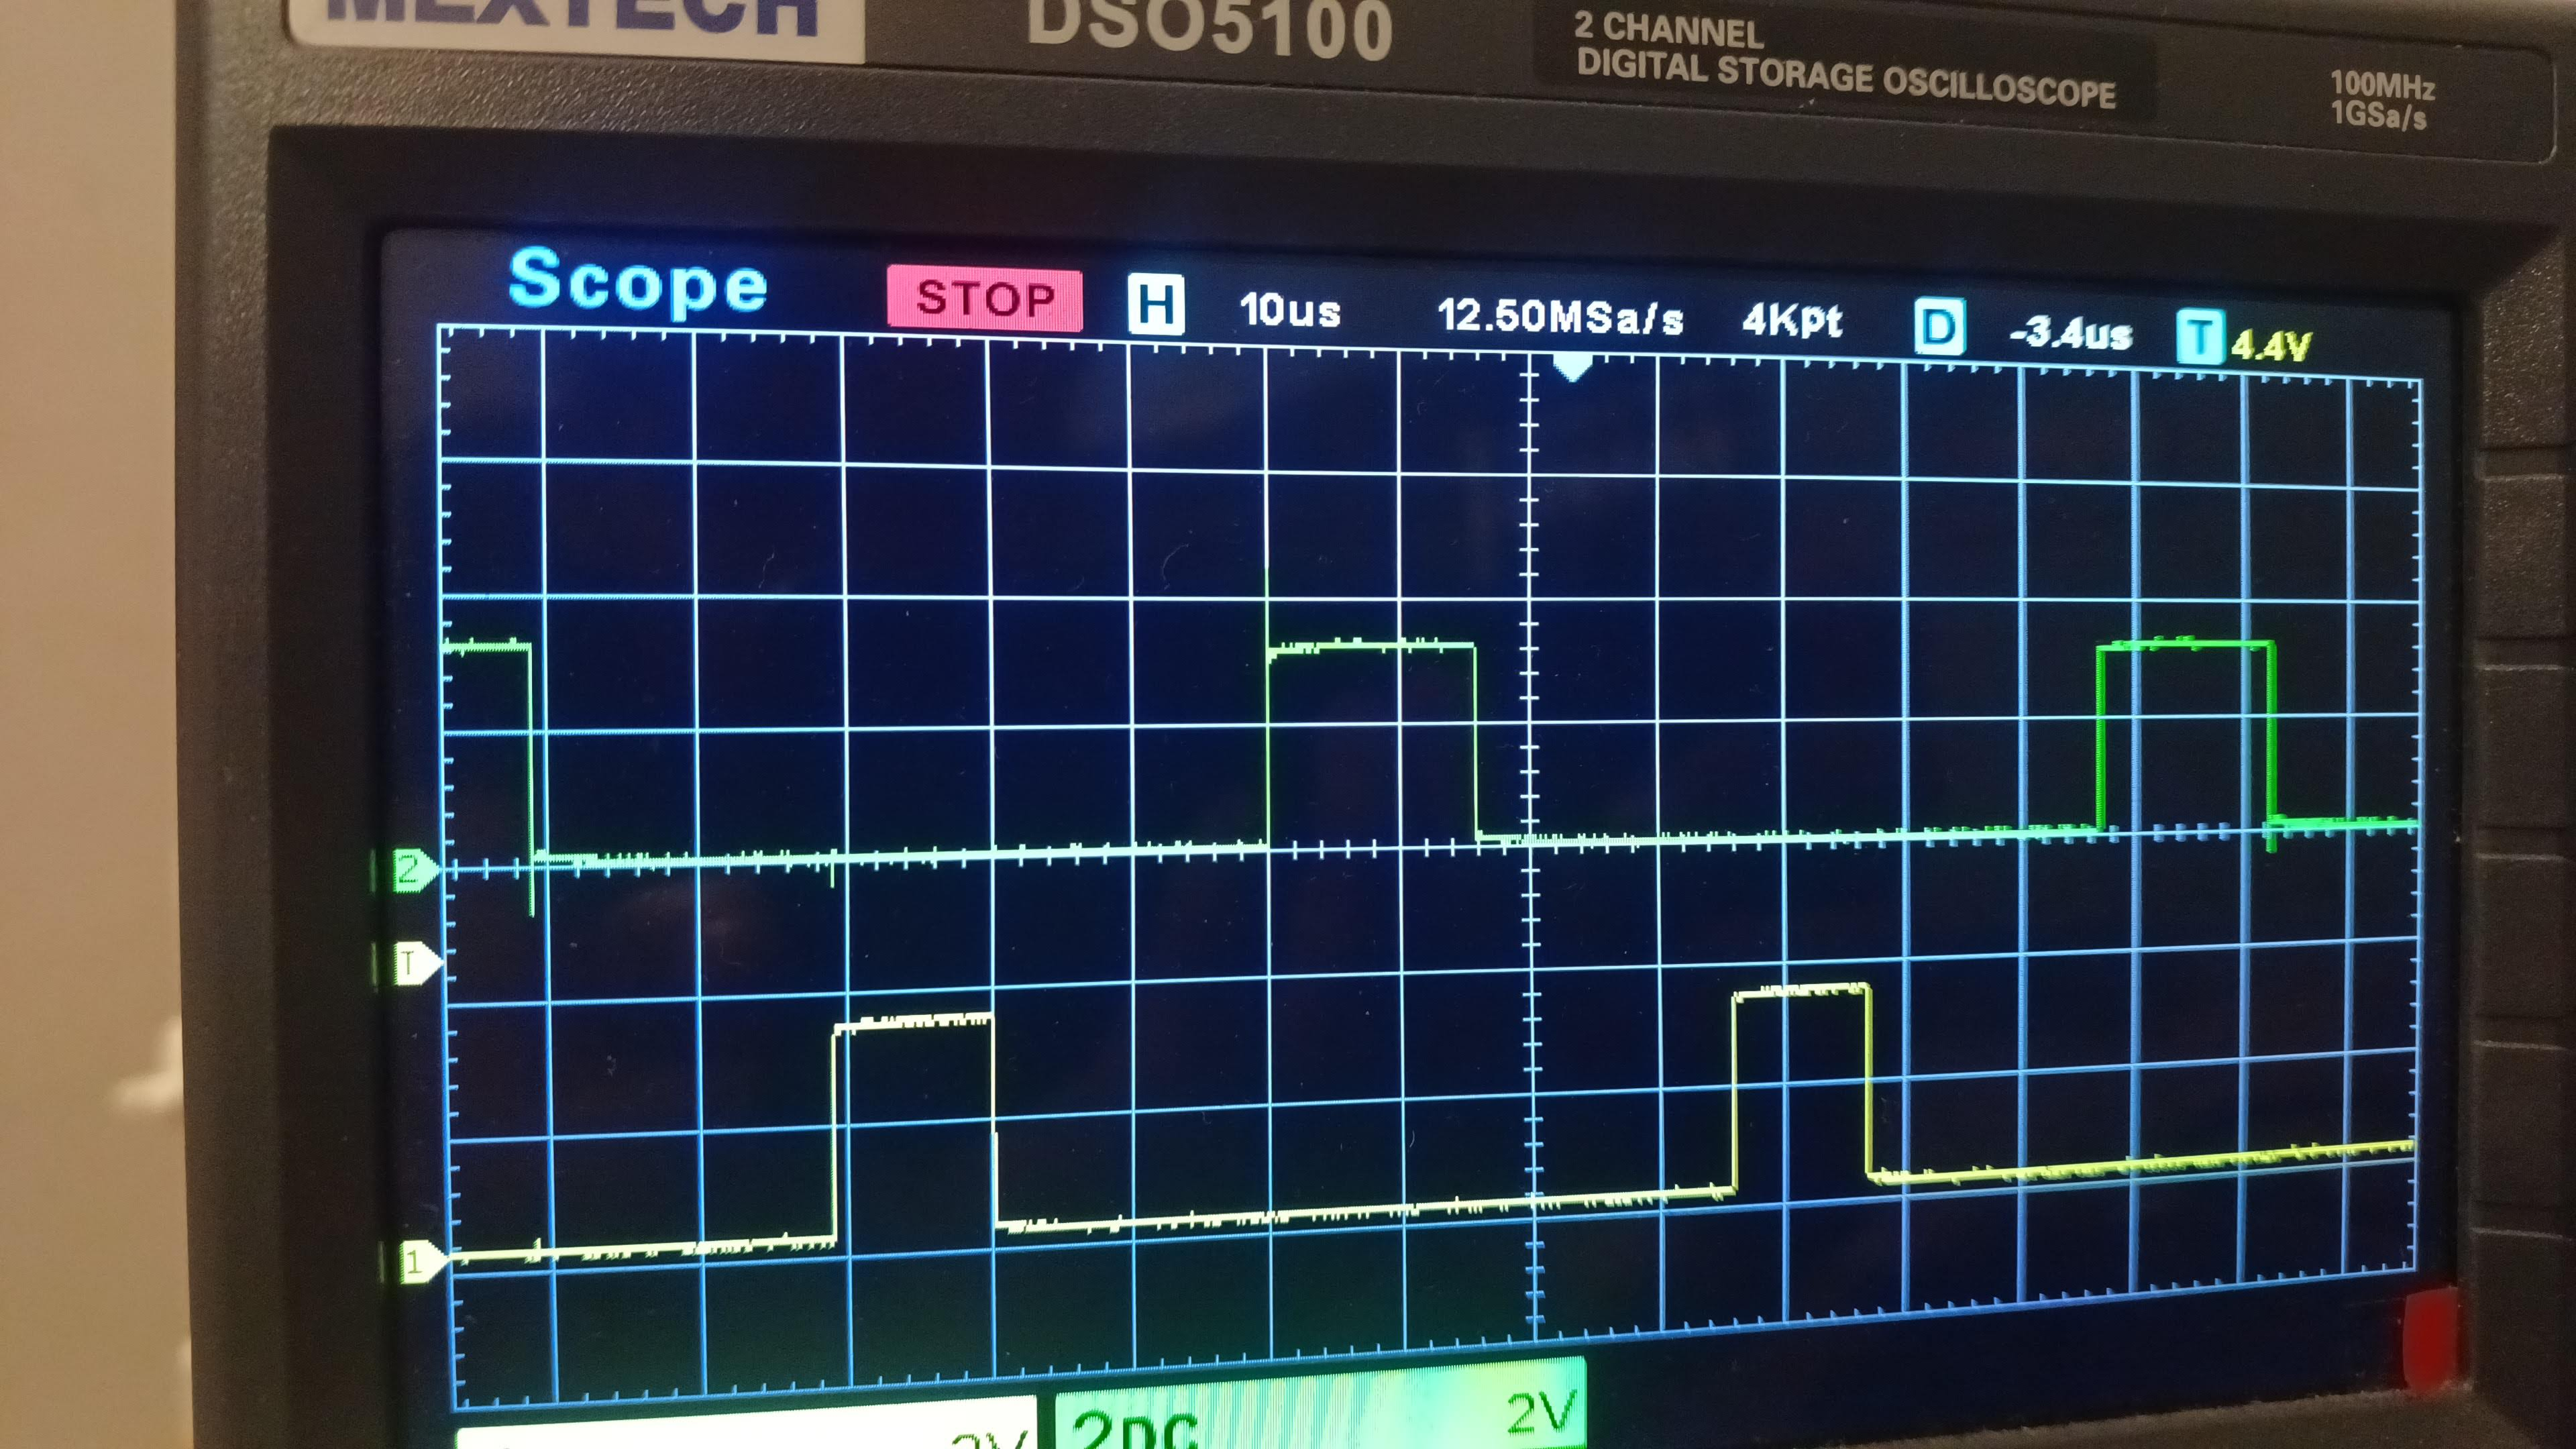
\includegraphics[width=4in]{sections/section6/images/SVPWM/DeadBand20Us.jpeg}}
		\caption{Dead band time}
	\end{figure}
\end{frame}





% Slide for DC Bus
\begin{frame}{DC Bus Setup}
	\begin{figure}
		\centering
		\fbox{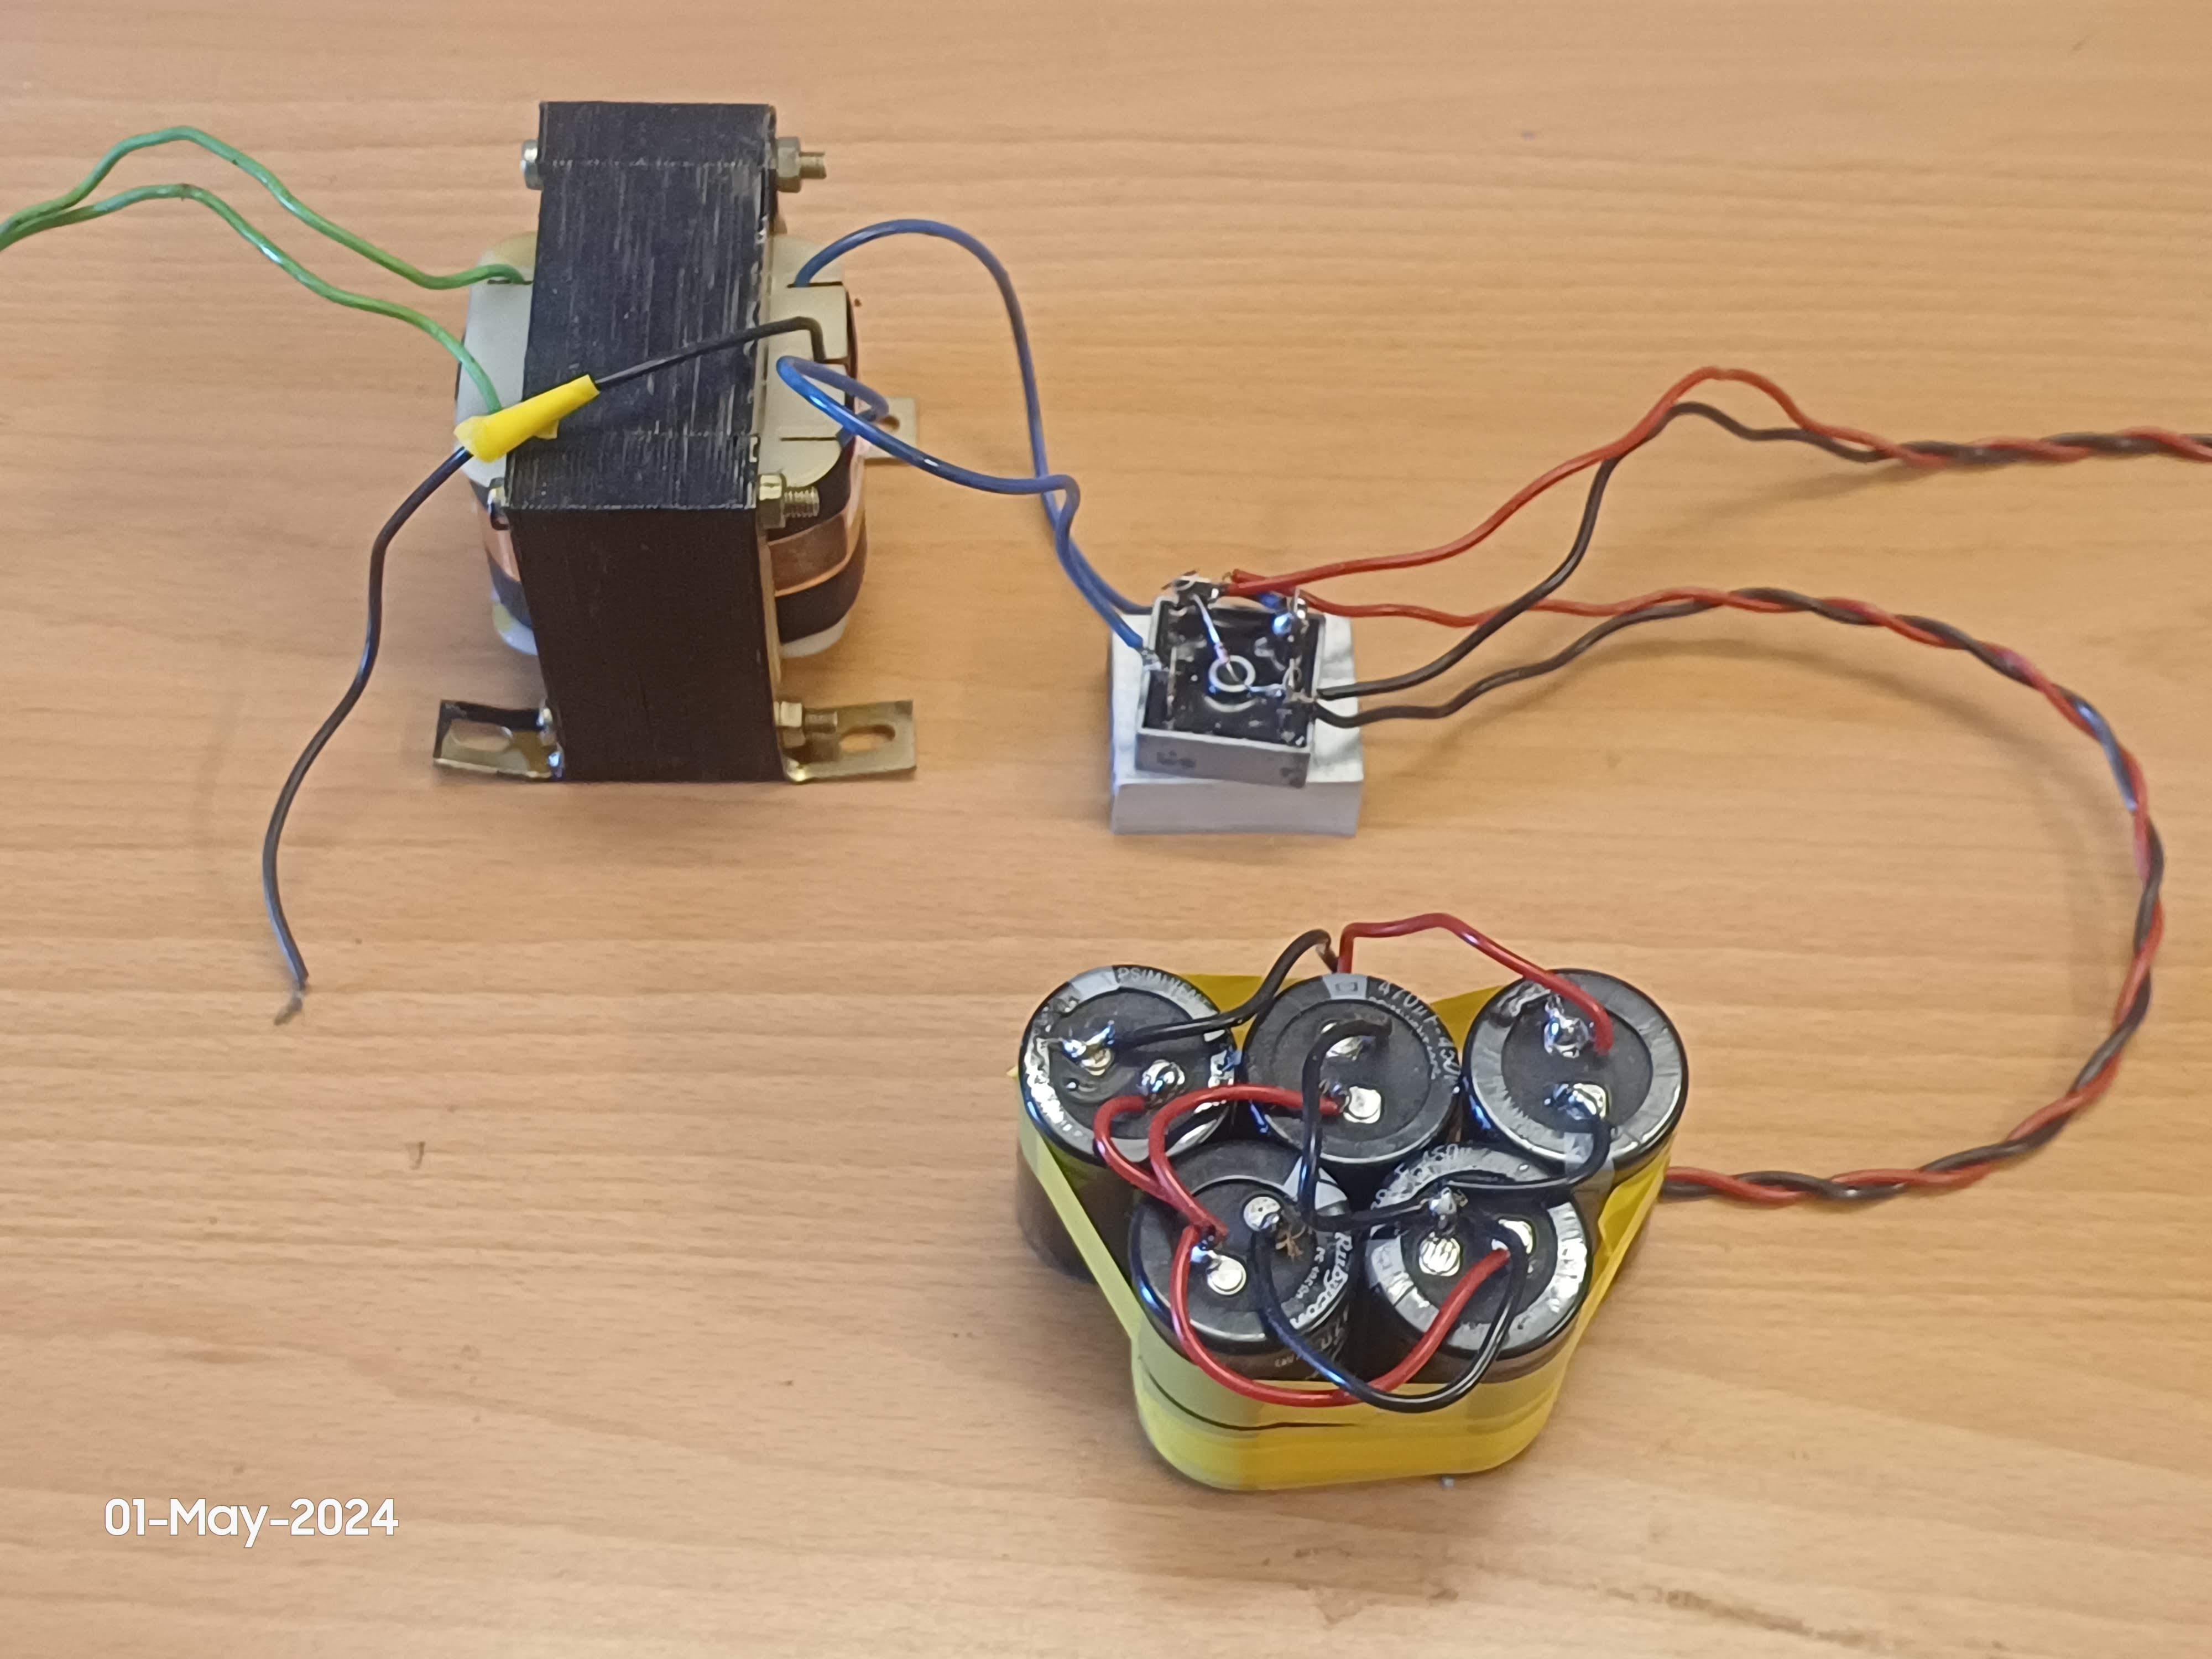
\includegraphics[width=3in]{sections/section6/images/hardwareSetup/DC bus rectifier transformer.jpg}
		}\caption{DC Bus Setup: 230V AC to 48V DC conversion with capacitor banks for stable power delivery}
	\end{figure}
\end{frame}

% Slide for Inverter and Controller
\begin{frame}{Inverter and Controller}
	\begin{figure}
		\centering
		\fbox{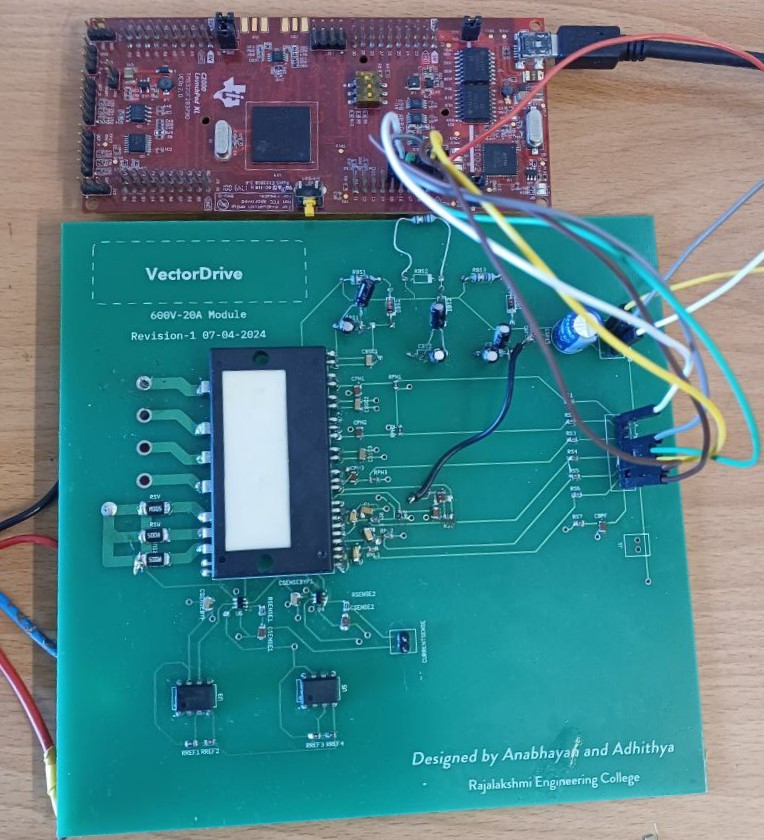
\includegraphics[width=2.3in]{sections/section6/images/hardwareSetup/IPM and C2000.jpg}
		}\caption{Inverter (FSAM20SH60A) and Controller (F28379D Launchpad) Setup}
	\end{figure}
\end{frame}

% Slide for Full Setup
\begin{frame}{Complete Hardware Setup}
	\begin{figure}
		\centering
		\fbox{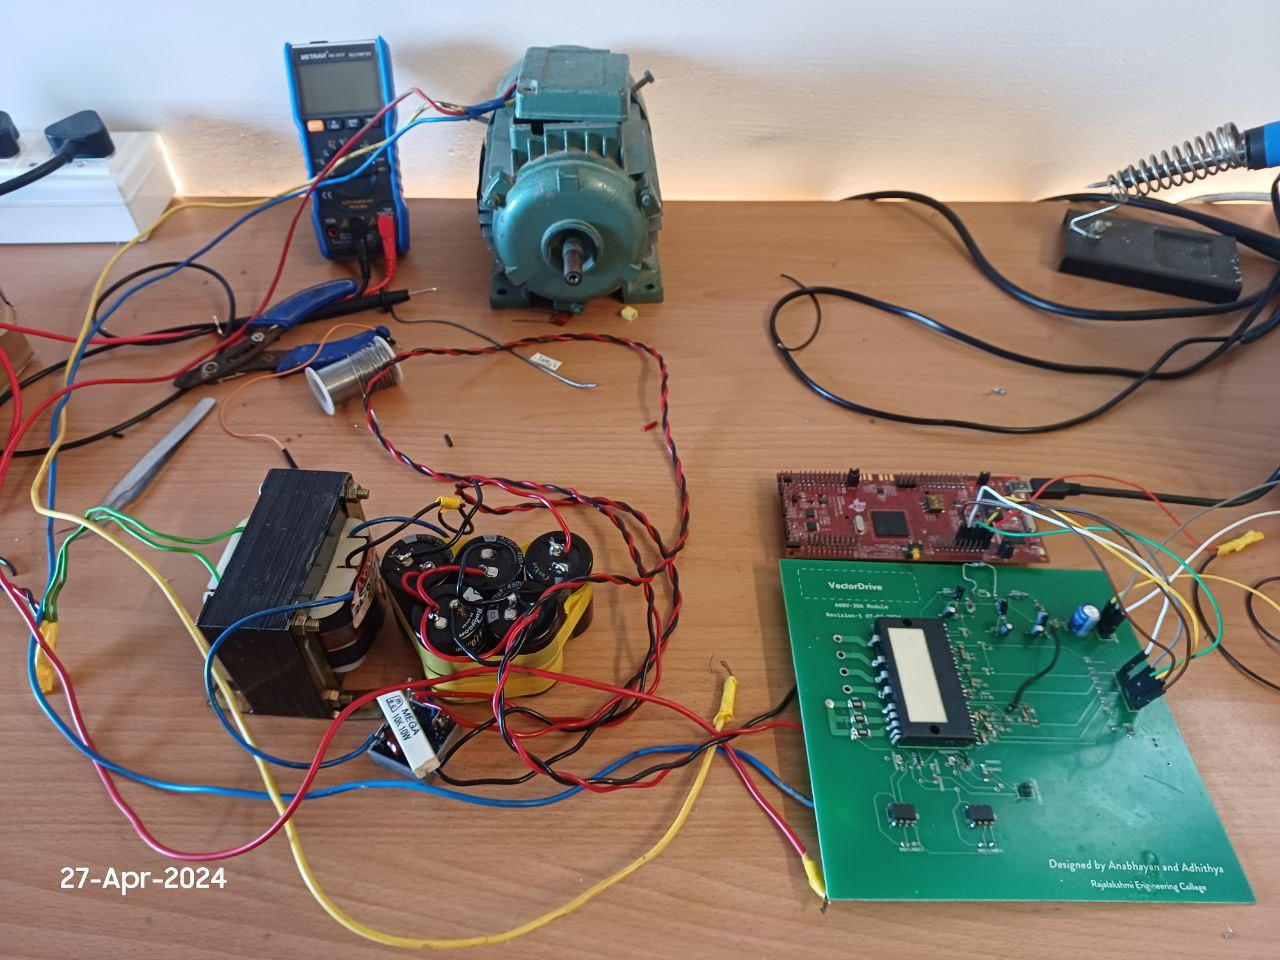
\includegraphics[width=3in]{sections/section6/images/hardwareSetup/fullSetupWithMotorAndIPM.jpg}
		}\caption{Experimental Setup for Motor Control System with Induction Motor, DC Bus, Inverter, and Controller}
	\end{figure}
\end{frame}

\begin{frame}{Challenges: False Positives from Fault Alarm}

	\begin{figure}
		\centering
		\fbox{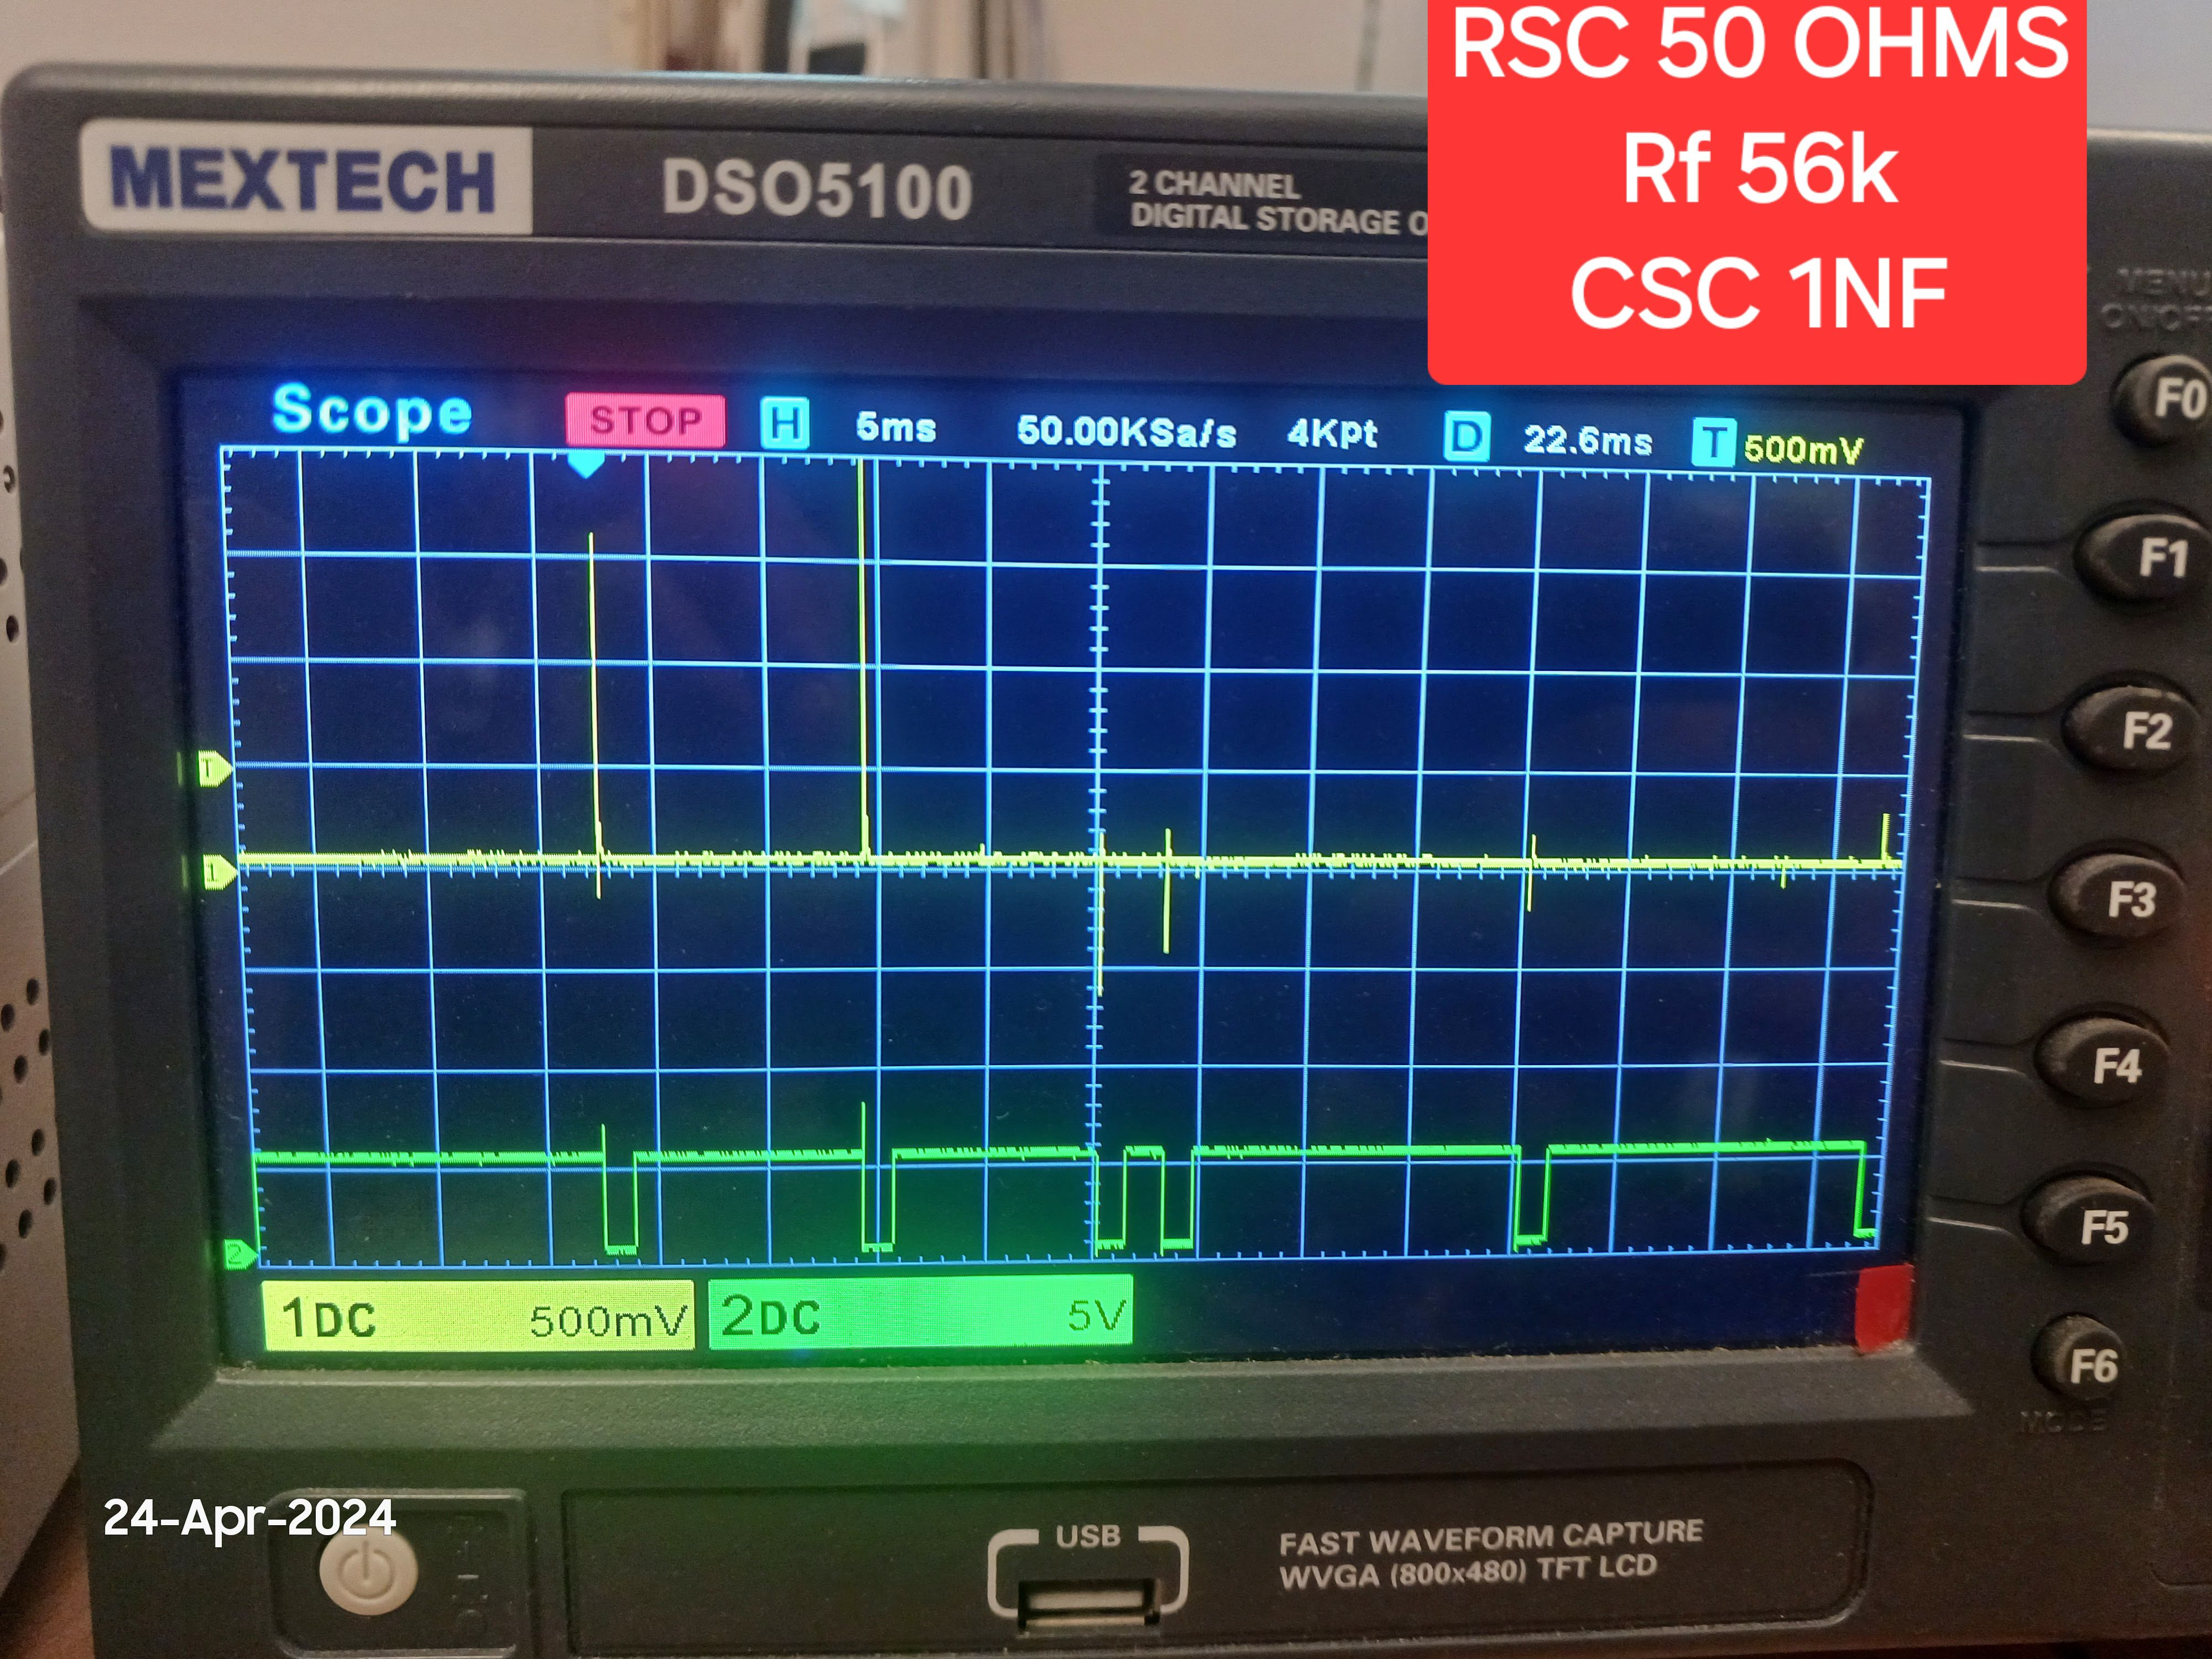
\includegraphics[width=4in]{sections/section6/images/hardwareSetup/VccNoiseAndFaultAlarm.jpg}
		}\caption{Vcc Noise and Fault Alarm Signal}
	\end{figure}

	\begin{itemize}
		\item Top waveform: Vcc voltage (power supply for IPM control)
		\item Bottom waveform: Fault alarm signal (triggered by noise on Vcc)
	\end{itemize}

\end{frame}
\begin{frame}{Mitigation Strategies}

	\begin{itemize}
		\item \textbf{Isolation Attempts:}
		      \begin{itemize}
			      \item Separate control and power stage grounds using separate transformers and rectifiers.
			      \item Temporarily shorted RSC and CSC pins to ground to assess external noise influence.
		      \end{itemize}
		\item \textbf{Noise Reduction Techniques:}
		      \begin{itemize}
			      \item Added metal film capacitors across the DC bus to suppress switching transients.
			      \item Reduced switching frequency to minimize voltage/current change rate and noise.
		      \end{itemize}
		\item \textbf{Future Considerations:}
		      \begin{itemize}
			      \item Further noise reduction through filtering on control signals and power supply lines.
			      \item Improved PCB layout to minimize noise coupling paths and optimize component placement.
		      \end{itemize}
	\end{itemize}

\end{frame}

\begin{frame}{Conclusion}

	\begin{itemize}
		\item \textbf{Achievements:}
		      \begin{itemize}
			      \item Successful simulation of FOC system demonstrating significant performance improvements.
			      \item Design and development of hardware setup including PCB design and component integration.
			      \item Identification and analysis of challenges related to noise and false alarms.
		      \end{itemize}
		\item \textbf{Challenges:}
		      \begin{itemize}
			      \item Persistent false positives from the IPM's fault alarm despite implemented mitigation strategies.
			      \item Limited hardware validation due to the unresolved fault alarm issue.
		      \end{itemize}
		\item \textbf{Future Work:}
		      \begin{itemize}
			      \item Explore additional noise reduction techniques and PCB layout optimization.
			      \item Investigate alternative IPM modules or fault detection mechanisms.
			      \item Implement and validate the closed-loop FOC system in hardware upon resolving the challenges.
		      \end{itemize}
	\end{itemize}

\end{frame}
\end{document}